% ----------------------------------------------------------------------
%                   LATEX TEMPLATE FOR PhD THESIS
% ----------------------------------------------------------------------

% based on Harish Bhanderi's PhD/MPhil template, then Uni Cambridge
% http://www-h.eng.cam.ac.uk/help/tpl/textprocessing/ThesisStyle/
% corrected and extended in 2007 by Jakob Suckale, then MPI-CBG PhD programme
% and made available through OpenWetWare.org - the free biology wiki


%: Style file for Latex
% Most style definitions are in the external file PhDthesisPSnPDF.
% In this template package, it can be found in ./Latex/Classes/
\documentclass[oneside,11pt]{Latex/Classes/PhDthesisPSnPDF}

%: Macro file for Latex
% Macros help you summarise frequently repeated Latex commands.
% Here, they are placed in an external file /Latex/Macros/MacroFile1.tex
% An macro that you may use frequently is the figuremacro (see introduction.tex)
\include{Latex/Macros/macros}

\DeclareMathAlphabet{\mathcal}{OMS}{cmsy}{m}{n}

%glossary ralated code
\usepackage[toc]{glossaries}
\renewcommand*{\glossaryentrynumbers}[1]{}
%\setlength{\glsdescwidth}{0.8\linewidth}
\makeglossaries

\glossarystyle{list}
\renewcommand*{\glsgroupskip}{}

\addbibresource[]{bibliography.bib}


% this file is called up by thesis.tex
% content in this file will be fed into the main document

% 1 = Entry name, e.g. abbreviation; 2 = Explanation
% You can place all explanations in this separate file or declare them in the middle of the text. Either way they will be collected in the glossary.

% required to print nomenclature name to page header
\newacronym{SLAM}{SLAM}{Simultaneous Localization And Mapping}
\newacronym{LRF}{LRF}{Laser Range Finder}
\newacronym{aLRF}{aLRF}{actuated Laser Range Finder}
\newacronym{NBV}{NBV}{Next Best Viewpoint}
\newacronym{FoV}{FoV}{Field of View}
\newacronym{ToF}{ToF}{Time of Flight}
%\newacronym{NNS}{NNS}{Nearest Neighbor Search}
\newacronym{EGI}{EGI}{Extended Gaussian Image}
%\newacronym{PCA}{PCA}{Principal Component Analysis}
\newacronym{MSE}{MSE}{Mean Square Error}
\newacronym{ICP}{ICP}{Iterative Closest Point}
\newacronym{NDT}{NDT}{Normal Distributions Transform}
\newacronym{3D-NDT}{3D-NDT}{Three-Dimensional Normal Distributions Transform}
\newacronym{MUMC}{MUMC}{Minimum Uncertainty Maximum Consensus}
\newacronym{IMU}{IMU}{Inertial Measurement Units}
\newacronym{GNSS}{GNSS}{Global Navigation Satellite Systems}
%\newacronym{EKF}{EKF}{Extended Kalman Filter}
%\newacronym{MLS}{MLS}{Multi-Level Surface}
\newacronym{PDF}{PDF}{Probability Density Functions}
%\newacronym{MLE}{MLE}{Maximum-Likelihood Estimation}
%\newacronym{P2D}{P2D}{Point-to-Distribution}
%\newacronym{FPFH}{FPFH}{Fast Point Feature Histograms}
%\newacronym{DIFT}{DIFT}{Depth-interpolated Image FeaTures}
\newacronym{RANSAC}{RANSAC}{RANdom SAmple Consensus}
\newacronym{SVM}{SVM}{Support Vector Machine}
\newacronym{PTU}{PTU}{Pan-Tilt Unit}
\newacronym{FILO}{FILO}{First-In-Last-Out}


%: ----------------------------------------------------------------------
%:                  TITLE PAGE: name, degree,..
% ----------------------------------------------------------------------
\ifpdf
    \pdfinfo { /Title  (PhD Thesis)
               /Creator (TeX)
               /Producer (pdfTeX)
               /Author (Benjamin Adler adler@informatik.uni-hamburg.de)
               /CreationDate (D:20140120)  %format D:YYYYMMDDhhmmss
               /ModDate (D:20140502)
               /Subject (robotics)
               /Keywords (Autonomous Robotics, Exploration, Mapping, SLAM) }
    \pdfcatalog { /PageMode (/UseOutlines)
                  /OpenAction (fitbh)  }
\fi

% ----------------------------------------------------------------------


\hyphenation{Sym-pa-tho-mi-me-ti-ka}
%\hyphenation{ent-"undungs-hemmende}
%\hyphenation{Ganz-k"or-per-ple-thys-mo-gra-phie}


% turn of those nasty overfull and underfull hboxes
\hbadness=10000
\hfuzz=50pt
%: --------------------------------------------------------------
%:                  FRONT MATTER: dedications, abstract,..
% --------------------------------------------------------------
%\makeglossaries
\begin{document}
% sets line spacing
\renewcommand\baselinestretch{1.0}
\baselineskip=14pt plus1pt

%: ----------------------- generate cover page ------------------------

\maketitle  % command to print the title page with above variables

%: ----------------------- tie in front matter ------------------------
%\frontmatter
\reviewers
%\include{0_frontmatter/dedication}
%\phantomsection
\chapter*{Change list}
\markboth{\MakeUppercase{Change list}}{}
\addcontentsline{toc}{chapter}{Change list}

\begin{itemize}
 \item Figure 3.2(b), the horizontal field of view has been corrected to 360 degrees.
 \item Algorithm 4.4, line 1, duplicate of Q <-- emptyset.
\end{itemize}
% Thesis Acknowledgements ------------------------------------------------
\phantomsection
\chapter*{Acknowledgements}
\markboth{\MakeUppercase{Acknowledgements}}{}
\addcontentsline{toc}{chapter}{Acknowledgements}

\if0
Doing a PhD was a long and exciting journey, which would not be possible without the help and support of many people. First of all I am most grateful to my supervisor Prof. Dr. Jianwei Zhang for giving me the opportunity to pursue a PhD at the University of Hamburg and providing me such a good and liberal academic environment. 

Next, I would like to extend my thanks to my daily supervisor and good friend Prof. Dr. Houxiang Zhang, whose support was always there for both technical and personal problems, not only in the first two years of my study when he was in Hamburg, but also for the second two years after he moved to {\AA}lesund. His constructive criticism helped focus my ideas and his constant encouragement kept me going in spite of many stumbling blocks on the road.    

Writing a dissertation is no easy task, but the same can be said of reviewing it. I would like to thank all the people who helped by reviewing parts of this work, especially my external reviewers --- Prof. Dr. Reinhard Koch and Dr. Peer Stelldinger. 

%I have to say, without your encouragement, I was almost going to drop when the traffic accident came to me while I had been ill for a long time. 

All the members of our TAMS group are greatly acknowledged, the time spent with you was wonderful. I own a great deal to Tatjana (Lu) Tetsis, thank you for helping me so much during the past time. My sincere thanks also go to Benjamin Adler for always being excited about my problems and ideas, always sharing his ideas with me, and the engaging discussions we had during and after work. 

I am grateful to my former colleagues from NuBot, Huimin Lu, Xiangke Wang, and Shaowu Yang are especially acknowledged, thanks a lot for valuable comments and suggestions on my conference and journal papers, as well as this dissertation. 

%I am thankful to all the people who helped by reviewing this work, they are Dr. Norman Hendrich, Shaowu Yang, Benjamin Adler, Weiwei Kong, and Jie Liang; especially my external reviewers --- Prof. Dr. Reinhard Koch and Dr. Peer Stelldinger.   

Being away from my family was not easy, however, many friends from Hamburg and other places provided another family away from home. I own special thanks to all of my friends. In this regard, Jianhua Zhang, Guoyuan Li, Gang Cheng, Bo Sun, and Weiwei Kong deserve special mention.

Finally, I would like to thank the people closest to me for their love and support --- my parents and brother, my girl friend Fang, especially to my little nephew who brings a lot of happy moments.  
\fi
% ------------------------------------------------------------------------

\vspace*{5mm}

\hfill Benjamin Adler

\hfill Hamburg, May 2014

\phantomsection
\chapter*{Abstract}
\markboth{\MakeUppercase{Abstract}}{}
\addcontentsline{toc}{chapter}{Abstract}

This paper introduces a custom-built unmanned aerial vehicle, capable of autonomous exploration in urban environments. It consists of a multicopter, an inertial navigation system and two 2D laser range finders. In addition to a description of the hardware architecture and individual components being used, the authors also discuss challenges and problems that arose during its construction as well as optimizations and workarounds applied in the course of its development.

Also presented is the software architecture, with a focus on a novel algorithm capable of generating multiple next best views (NBVs), sorted by achievable information gain. Although being designed for application on airborne platforms in urban environments, it works directly on raw point clouds and thus can be used with any sensor generating spatial occupancy information (e.g. LIDAR, RGBD- or time-of-flight-cameras). To satisfy constraints introduced by real-time operation on UAVs, the algorithm is implemented on a highly parallel SIMD architecture and benchmarked using GPUs from multiple hardware generations, using data from real flights. It is also compared against the previous, CPU-based proof of concept.

As the underlying hardware imposes limitations with regards to memory access and concurrency, necessary data structures and further performance considerations are explained in detail.

Open-source code for this paper is available at http://www.github.com/benadler/octocopter/.
\phantomsection
\chapter*{Kurzfassung}
\markboth{\MakeUppercase{Kurzfassung}}{}
\addcontentsline{toc}{chapter}{Kurzfassung}

Die vorliegende Dissertation behandelt ...
%: ----------------------- contents ------------------------
\setcounter{secnumdepth}{3} % organisational level that receives a numbers
\setcounter{tocdepth}{3}    % print table of contents for level 3
\tableofcontents            % print the table of contents
\addtocontents{toc}{\protect{\pdfbookmark[0]{\contentsname}{toc}}}
% levels are: 0 - chapter, 1 - section, 2 - subsection, 3 - subsection
%: ----------------------- list of figures/tables ------------------------
\listoffigures	% print list of figures
\newpage\thispagestyle{empty}
\listoftables  % print list of tables
\newpage\thispagestyle{empty}

%\glsaddall
\printglossaries
\newpage\thispagestyle{empty}


\begin{multicols}{2} % \begin{multicols}{#columns}[header text][space]
\begin{footnotesize} % scriptsize(7) < footnotesize(8) < small (9) < normal (10)
\printnomenclature[1.5cm] % [] = distance between entry and description
\label{nom} % target name for links to glossary

\end{footnotesize}
\end{multicols}

%: --------------------------------------------------------------
%:                  MAIN DOCUMENT SECTION
% --------------------------------------------------------------

% the main text starts here with the introduction, 1st chapter,...
\mainmatter
%: ----------------------- subdocuments ------------------------
% Parts of the thesis are included below. Rename the files as required.
% But take care that the paths match. You can also change the order of appearance by moving the include commands.

\begin{spacing}{1.5}

%: ----------------------- introduction file header -----------------------
\chapter{Einleitung}
\label{einleitung}
%\epigraph{Singen ist die Sprache der Wahrheit}{Sting}
% the code below specifies where the figures are stored
\ifpdf
    \graphicspath{{1_introduction/figures/PNG/}{1_einleitung/figures/PDF/}{1_einleitung/figures/}}
\else
    \graphicspath{{1_einleitung/figures/EPS/}{1_einleitung/figures/}}
\fi

% ----------------------------------------------------------------------
%: ----------------------- introduction content -----------------------
% ----------------------------------------------------------------------
In den letzten Jahrzehnten ist die Zahl der an Chronisch obstruktiver Lungenerkrankung (COPD= chronic obstructive pulmonary disease) leidenden Patienten rapide angestiegen - mittlerweile sind bereits rund 340 Millionen Menschen weltweit an COPD erkrankt. Sie steht momentan noch an vierter Stelle der häufigsten Todesursachen, laut der WHO soll sie bis 2030 sogar auf die dritte Stelle aufsteigen. Es handelt sich hierbei um eine nicht vollständig reversible und progrediente Lungenerkrankung, bei welcher die Patienten unter einer Obstruktion der Atemwege durch eine chronische Entzündung leiden. Dies geht einher mit häufiger Atemnot und starkem Auswurf.
Es wurde jedoch noch kein Medikament gefunden, dass die Erkrankung heilen oder wenigstens das Fortschreiten aufhalten kann. Dies mag u.a. der Tatsache geschuldet sein, dass die Forschung auf diesem Gebiet noch vergleichsweise jung ist. Aktuelle Forschungsergebnisse lassen jedoch auf eine Verbesserung der medikamentösen Therapie hoffen.

In der Behandlung kommen derzeit in erster Linie Pharmazeutika sowie Raucherentwöhnung, Atemtherapie, Bewegungstherapie und Entspannungstechniken wie z.B. autogenes Training zum Einsatz. In einigen Rehabilitationskliniken wird zudem psychologische Beratung angeboten, welche Patienten bei Bedarf in Anspruch nehmen können.

Viele Patienten sind leider nach wie vor nur sehr mangelhaft über ihre Erkrankung aufgeklärt und nehmen nur selten präventive therapeutische Angebote in Anspruch. Daraus resultiert jedoch oftmals ein Verhalten, dass nicht nur zur Verschlechterung der Erkrankung sondern auch zur Ausbildung von Komorbiditäten wie Herz-Kreislauf-Erkrankungen aber auch zu Depression und Angststörungen führt. Ein wichtiger Aspekt ist hierbei die Vermeidung von symptomverstärkenden Tätigkeiten (s.g. „Fear Avoidance“). Der Lungeninformationsdienst  berichtet, dass ca. 40\% der COPD-Patienten unter einer depressiven Symptomatik leide und fordert auf seiner Webseite, dass „eine psychotherapeutische Behandlung […] deshalb ein fester Bestandteil der COPD Therapie sein“ sollte. Auch an anderen Stellen, insbesondere bei Fachärzten, scheint dieser Aspekt stärker ins Bewusstsein zu rücken. Schaut man sich jedoch beispielsweise auf den Internetseiten der führenden pneumologischen (Reha-)Kliniken um, ist die psychologische Betreuung noch recht mangelhaft und die Krankheitsbewältigung i.S. einer psychotherapeutischen Begleitung noch kaum in die Behandlungskonzepte eingebettet. 

Ein weiterer interessanter Bereich in Bezug auf die nicht-medikamentöse Begleitbehandlung findet sich meines Erachtens in der neueren Singforschung. In unterschiedlichen Studien (siehe \ref{copd_in_der_singforschung}) wurde der Effekt von Singen auf die Lebensqualität und den Krankheitsfortschritt von COPD-Patienten untersucht. Dabei zeigte sich vor allem, dass sich die Lebensqualität signifikant steigerte, insbesondere durch die positiven Erfahrungen, in Gemeinschaft zu sein. Meine Vermutung ist zudem, dass eine Steigerung der Lebensqualität in diesem Fall auch eng mit der verstärkten Aktivierung der Selbstwirksamkeit verbunden sein könnte, welche aus der Erfahrung resultiert, dass die eigene Stimme trotz der Schwere der Erkrankung durch die eigene Kraft zum Klingen gebracht werden kann und die Atmung wieder mehr in der eigenen Kontrolle liegt. So könnte das Gefühl des „Ausgeliefertseins“ gegenüber den Krankheits-immanenten Symptomen wie plötzlicher Atemnot und Abnahme körperlicher Belastbarkeit  sukzessive verringert werden.

Diese beiden Aspekte, der Bedarf an psychotherapeutischer Begleitung u.a. für die Krankheitsbewältigung sowie zur Prävention vor Komorbiditäten als auch die positiven Wirkungen der Arbeit mit der Stimme, insbesondere dem Singen, möchte ich in dieser Masterarbeit konzeptionell zusammenbringen.

Im Folgenden werden die Erkrankung "COPD" und "Musiktherapeutische Stimmarbeit" als solche getrennt voneinander dargestellt, um so daran anschließend Überlegungen für die musiktherapeutische Arbeit mit COPD-Patienten entwickeln zu können.

Ein umfassendes Verständnis für die Bedürfnisse aber auch die krankheitsbedingten Belastungen von COPD-Patienten ist m.E. für die Arbeit mit diesem Klientel unerlässlich, um sie angemessen unterstützen zu können. Dafür erscheint es mir wichtig, unterschiedliche Aspekte der Erkrankung von der Pathologie über die Diagnostik zu Behandlungsmöglichkeiten etwas ausführlicher zu beleuchten. Insbesondere dem Gesichtspunkt "Komorbiditäten" wird im folgenden Kapitel besondere Aufmerksamkeit gewidmet, da dieser für die am Ende erläuterten konzeptionellen Überlegungen eine wichtige Grundlage bildet.

Da der Ansatz von Sabine Rittner sehr hilfreich und passend für die in dieser Masterthesis angestrebten konzeptionellen Überlegungen für die Arbeit mit COPD-Patienten scheint, wird unter \ref{chapter:musiktherapeutische_stimmarbeit} vielfach auf ihre Publikationen zurückgegriffen, um ein theoretisches Gerüst in Bezug auf die musiktherapeutische Stimmarbeit aufzubauen.

Im Kapitel "konzeptionellen Überlegungen" unter \ref{chapter:konzeptionelle_ueberlegungen} werden die eigenen Ideen und Ableitungen aus der für das Thema relevanten Literatur für die musiktherapeutische Arbeit mit COPD-Patienten beschrieben. Es wird erläutert, weshalb ein musiktherapeutisches Konzept in der hier beschriebenen Form sinnvoll erscheint. Diese Überlegungen beruhen neben der literarischen Auseinandersetzung sowohl auf Gesprächen mit Fachärzten und Fachtherapeuten, welche mit COPD-Patienten arbeiten als auch mit Betroffenen. Diesen sehr hilfsbereiten Gesprächspartnern, u.a. Wolfgang Bossinger (Musiktherapeut), Monika Wiese (Musiktherapeutin), Maria Weiser (Atemtherapeutin), Matthias Groth (Atemtherapeut), Dr. med. Sven Phillip Aries (Elbpneumologie) und Dr. med. Hans Klose (Oberarzt - Leiter der Sektion Pneumologie des Universitätsklinikums Hamburg Eppendorf) möchte ich hiermit meinen Dank aussprechen. Zudem sei meinen sehr engagierten Korrektorinnen und meinem Partner für ihre großartige Unterstützung gedankt, ohne welche diese Arbeit nicht diese nun vorliegende Gestalt hätte annehmen können.

\newpage\thispagestyle{empty}
\ifpdf
\graphicspath{{2_chronisch_obstruktive_lungenerkrankung/figures/PNG/}{2_chronisch_obstruktive_lungenerkrankung/figures/PDF/}{2_chronisch_obstruktive_lungenerkrankung/figures/}}
\else
\graphicspath{{2_chronisch_obstruktive_lungenerkrankung/figures/EPS/}{2_chronisch_obstruktive_lungenerkrankung/figures/}}
\fi

\chapter{Chronisch obstruktive Lungenerkrankung (COPD)}
\label{chapter:copd}

Die Chronisch obstruktive Lungenerkrankung, auf englisch Chronic Obstructive Pulmonary Disease (COPD) genannt, ist trotz ihrer starken Verbreitung noch vielen Menschen nicht bekannt.
Bei der COPD handelt es sich um eine chronische Lungenkrankheit mit progredienter Atemwegsverengung; sie gilt als die häufigste Erkrankung der Atmungsorgane (Darstellung der Atmungsorgane siehe Abbildung \ref{fig:atemsystem}). 


\begin{figure}
 \centering
  \includegraphics[width=1.0\textwidth]{atemsystem}
  \caption{Aufbau des Atmungssystems bis in die kleinsten Lungenstrukturen, die Alveolen. Eine Abbildung des Zwerchfells findet sich in Kapitel \ref{chapter:musiktherapeutische_stimmarbeit} (entnommen aus \cite[178]{schoppmeyer2012})}
  \label{fig:atemsystem}
\end{figure}

COPD ist ein Sammelbegriff für die chronisch obstruktive Bronchitis und das Lungenemphysem, welche entweder einzeln oder gemeinsam auftreten \autocite[vgl.][153]{lorenz2009}. Die COPD resultiert aus einer langfristigen Entzündung der Atemwege, welche durch ständige Belastung mit Zigarettenrauch, aber auch Umweltfaktoren, Staubpartikeln und giftigen Dämpfen entsteht. Ätiologisch wird davon ausgegangen, dass 80-90\% der COPD-Patienten die Erkrankung aufgrund von Nikotinabusus entwickelt haben; das sind in etwa 15\% der Zigarettenraucher\autocite[vgl.][154]{lorenz2009}. 

Als ein wichtiges Diagnosemerkmal gilt die Atemnot (Dispnoe), welche aus der Obstruktion der Bronchien resultiert (siehe Abbildung \ref{fig:copd_emphysem}). Diese wird durch drei Faktoren ausgelöst: 

\begin{enumerate}
\item Verkrampfung der Bronchialmuskulatur (Bronchospasmus)
\item Anschwellen der Schleimhaut in den Bronchien (Ödem)
\item Krankhaft erhöhte Schleimproduktion (Hyperkrinie) aufgrund einer dauerhaften Entzündung der Atemwege (chronische Bronchitis)
\end{enumerate}

Aufgrund der Bewegungseinschränkung durch die Hyperkrenie werden die Zilien - kleine Flimmerhärchen in den Bronchien - immer mehr daran gehindert, Schadstoffe aus der Lunge hinaus zu befördern. Dieser Prozess führt über einen längeren Zeitraum zur Zerstörung der Flimmerhärchen und somit zu einem größeren Exazerbationsrisiko (siehe unten).
Die Luftnot tritt im Anfangsstadium nur unter Belastung auf, später auch im Ruhezustand \autocite[vgl.][6f.]{lorenz2009}. Die allgemeine Symptomatik umfasst morgendlichen Kopfschmerz, Gewichtsverlust, welcher auf verstärkte Atemarbeit und systemische Entzündungsreaktionen zurückzuführen ist, zunehmenden Leistungsabfall, Einflussstauung, Ödeme der unteren Extremitäten und weiter abnehmende Belastbarkeit aufgrund des s.g. Cor pulmonale (Lungenherz, s. weiter unten).
Eine chronisch obstruktive Lungenerkrankung liegt laut WHO-Definition dann vor, wenn sowohl Husten und Auswurf über wenigstens als 3 Monate in mindestens 2 aufeinander folgenden Jahren bestehen und somit als chronisch anzusehen sind, als auch andere Krankheiten wie z.B. Bronchiektasen, Staubbelastung, cystische Fibrose, Asthma, Fremdkörper u.a. im Vorfeld ausgeschlossen werden konnten \autocite[vgl.][71]{koehler2010}. 

\begin{figure}
 \centering
  \includegraphics[width=0.6\textwidth]{copd_emphysem}
  \caption{Die Abbildung zeigt die typischen pneumologischen Veränderungen bei COPD und Lungenemphysem. Oben: Querschnitt eines gesunden (links) und eines entzündeten Bronchus. Unten: Die rechte Darstellung der Alveolen zeigt die krankhaft veränderte Struktur der Alveolarwände bei einem Lungenemphysem \cite[vgl.][16]{lingemann2014})}
  \label{fig:copd_emphysem}
\end{figure}

Das Lungenemphysem ist das Resultat länger andauernder Entzündungsreaktionen auf o.g. mögliche externe Partikel. Durch entzündliche Prozesse werden die Zellwände in den Alveolen (Lungenbläschen, siehe Abbildung \ref{fig:copd_emphysem}) zerstört. Hierfür sind Proteasen zuständig, die beim Eindringen von schädlichen Stoffen in die Lunge durch das Immunsystem freigesetzt werden. So genannte Antiproteasen können jedoch vor der Zerstörung der Alveolarwände schützen. Diese werden für normal körpereigen produziert; hierzu gehört u.a. das Alpha-1-Antitrypsin. Einige Patienten leiden jedoch unter einem genetische bedingen Alpha-1-Antrypsinmangel, wodurch ein erhöhtes Risiko für die Ausbildung eines Lungenemphysems besteht.
Das bedeutet, dass sich mit weiterbestehender Entzündung die Anzahl der für den Sauerstoff-Kohlendioxid-Austausch notwendigen Alveolen verringert und sich die Lufträume in der Lunge vergrößern. Dadurch wird nach und nach die Lungenelastizität eingeschränkt, was eine Überdehnung der Lunge (Hyperinflation) mit Minderdurchblutung und einem irreversiblen Schwund an Lungengewebe als auch eine Einschränkung der Atemfunktion nach sich zieht. Dies geschieht jedoch nicht nur durch die degenerativen Prozesse in einem Lungenlappen, sondern auch durch funktionelle Beeinträchtigung anderer umliegender, gesunder Lungenlappen aufgrund der partiellen Überblähung. Auch andere Organe können möglicherweise beschädigt werden. Denn bei Nichtbehandlung des Emphysems kommt es zu einer erhöhten Pumpleistung des Herzmuskels und so über längere Zeit zu einer Schädigung desselben, da dieser nun mehr Blut transportieren muss, um die Organe ausreichend mit Sauerstoff zu versorgen. So ist vor allem das Endstadium der COPD gekennzeichnet durch das Auftreten des so genannten Cor Pulmonare, dem Lungenherz. Hiermit ist die Rechtsherz-Insuffizienz gemeint, bei welcher die rechte Herzkammer aufgrund des Blutstaus durch den langsameren Sauerstoff-Kohlendioxid-Austausch in den Lungen immer größer wird und an Leistungskraft verliert \autocite[vgl.][e10]{vogelmeier2007}.

Bei Fortschreiten der COPD kommt es immer wieder zu Exazerbationen, das heißt zu akuten Verschlechterungen der alltäglichen Krankheitssymptome, was zu Symptomen wie Atemnot, Husten, vermehrter Sputummenge oder Fieber führen kann. Sie resultieren zu 60-70\% aus einer Infektion der Lunge oder nichtinfektiösen Ursachen wie akuter Luftverschmutzung oder Verschlechterung von Begleiterkrankungen und sollten daher zeitnah behandelt werden.

Das Auftreten der COPD nimmt mit dem Alter zu, dabei kommt es ab dem 50. Lebensjahr zu einem rapiden Anstieg der Prävalenz. Im siebten Dezennium ist die Spitze des Auftretens mit etwa 10\% bei Männern und ca. 5\% bei Frauen erreicht\autocite[vgl.][153]{lorenz2009}. Nach Köhler/Schönhofer/Voshaar (2010) sei Vorsicht geboten bei dem Einbezug von Statistiken in diesem Bereich, da die verfügbaren Daten zur Prävalenz der COPD sehr von dem untersuchten Kollektiv bzw. den Altersgruppen abhängen (vgl. ebd., 72). Insgesamt gehen sie jedoch von folgenden Zahlen aus: Etwa 10\% der deutschen Bürger ab dem 40. Lebensjahr seien davon betroffen, wobei ca. 10\% dieser Patientenkohorte einen höheren Schweregrad (siehe Tabelle \ref{tab:copd_schweregrade})  aufweisen. Es wird davon ausgegangen, dass den Hausärzten nur etwa bei der Hälfte der Patienten die Erkrankung bekannt ist.
In Bezug auf die Mortalität gilt bei ca. 3,5\% aller Todesfälle COPD als die Haupttodesursache. Allerdings ist sie bei ca. 4,5\% der Todesfälle mitverursachend. Es wird davon ausgegangen, dass COPD auf der Liste der häufigsten Todesursachen in den nächsten 6 Jahren weltweit von dem 4. auf den 3. Platz aufsteigen wird.
Laut der COPD-Leitlinie besteht eine hohe sozioökonomische Belastung durch die steigende Zahl an COPD-Fällen. In der Hochrechnung von Krankenhausstatistiken seit 1996 wurden für obstruktive Atemwegserkrankungen 2,7 Mio. Krankenhaustage erfasst. Einen Großteil macht hierbei die Behandlung chronischer Bronchitis und ihrer Folgen aus. Auch die von der AOK hochgerechneten jährlichen Krankheitstage in Höhe von 25 Mio. aufgrund der chronischen Bronchitis sind immens. Sie entsprechen volkswirtschaftlichen Gesamtkosten von etwa 5,93 Mrd. Euro jährlich \autocite[vgl.][e4]{vogelmeier2007}.

Um das Krankheitsbild, Diagnostik und Therapie weltweit zu vereinheitlichen, wurde der o.g. englische Begriff eingeführt. Eine globale Initiatve, welche 2001 von der Weltgesundheitsorganisation (WHO) und den National Institutes of Health (NIH) gegründet wurde, hat zusätzlich dazu beigetragen, dass weltweit eine einheitliche Leitlinie, die s.g. GOLD-Leitlinie, zum Tragen kommt. Die Erkrankung wird hiernach in vier Schweregrade eingeteilt, die sich an dem gemessenen Ausatemvolumen orientieren. Einige Autoren, darunter Köhler/Schönhofer/Voshaar \autocite[vgl.][75]{koehler2010}, bewerten diese Leitlinie jedoch als einen Rückschritt, da diese das Krankheitsbild in Bezug auf seine Pathophysiologie zu sehr vereinfache.

Diese Einteilung wird jedoch in der Praxis nach wie vor vorgenommen, weshalb sie an dieser Stelle dargestellt werden soll.

In den GOLD-Leitlinien wird zwischen 4 Stadien unterschieden. Für die Einteilung kommen 2 Werte der Lungenfunktionsprüfung (siehe Kapitel \ref{diagnostik}) zum Tragen. Der erste Wert, das forcierte exspiratorische Volumen ($FEV_{1}$) gibt Auskunft darüber, wieviel Luft eine Person innerhalb einer Minute forciert ausatmen kann. Für eine Einstufung wird der $FEV_{1}$-Wert eines Patienten mit Soll- bzw. Normalwerten verglichen, welche wiederum abhängig von Geschlecht, Alter und Körpergröße des Patienten sind. Dieser Wert gilt in der Regel als Indikator für die Schwere der Erkrankung. In diesem Zusammenhang ist auch das Verhältnis zwischen der inspiratorischen Vitalkapazität (Einatemvolumen) und dem $FEV_{1}$ für die Diagnosestellung wichtig (siehe Tabelle \ref{tab:copd_schweregrade}). Bei der leichtgradigen COPD (Schweregrad I) besteht die Atemwegsobstruktion ohne eine signifikante $FEV_{1}$-Verminderung. Patienten in diesem Stadium berichten über chronischen Husten und Auswurf, bemerken jedoch meist noch keine Einschränkung ihrer Lungenfunktion. Beim Schweregrad II besteht neben der Atemwegsobstruktion bereits eine geringe $FEV_{1}$- Verminderung und die kranksheitsspezifischen Symptome, insbesondere Dyspnoe unter Belastung, nehmen zu. Die schwere COPD (Schweregrad III) ist charakterisiert durch eine höhergradige $FEV_{1}$-Verminderung, das heißt $FEV_{1}$-Werten zwischen 30\% und 50\% des Soll. Es besteht jedoch nur eine geringe oder keine Korrelation zwischen dem Ausmaß der Dyspnoe und dem Schweregrad der Lungenfunktionseinschränkung. Für den Schweregrad IV gilt ein $FEV_{1}$-Wert von $\leq$ 30\% Soll als ausschlaggebend. Bei einer gleichzeitigen respiratorischen Insuffizienz darf für die Einteilung in den Schweregrad IV der $FEV_{1}$-Wert $<$50\% soll betragen \autocite[vgl.][e8]{vogelmeier2007}.

\begin{table}
\centering
\begin{tabular}{lp{10cm}}
	\textbf{Schweregrad} & \textbf{Kriterien} \\
	\hline \hline
	I (leicht) & $FEV_{1} \ge 80\% Soll, FEV_{1}/VC < 70\%$ \newline mit/ohne Symptomatik (Husten, Auswurf) \\
	\hline
	II (mittel) & $50\% Soll \le FEV_{1} < 80\% Soll, FEV_{1}/VC < 70\%$ \newline mit chronischen Symptomen/ohne chronische Symptome (Husten, Auswurf, Dyspnoe) \\
	\hline
	III (schwer) & $30\% Soll < FEV_{1} < 50\% Soll, FEV_{1}/VC < 70\%$ \newline mit chronischen Symptomen/ohne chronische Symptome (Husten, Auswurf, Dyspnoe) \\
	\hline
	IV (sehr schwer) & $FEV_{1} \le 30\% Soll, FEV_{1}/VC < 70\%$ oder \newline $FEV_{1} < 50\% Soll$ plus chronische respiratorische Insuffizienz \\
	\hline
\end{tabular}
\caption{Schweregradeinteilung der COPD, aus \autocite[e9]{vogelmeier2007}}
\label{tab:copd_schweregrade}
\end{table}

Eine neuere, multidimensionale Schweregradbeurteilung stellt der s.g. BODE-Index dar (siehe Anhang). Dieser bezieht in seine Bewertung den Body-Mass-Index (B), die $FEV_{1}$-Einschränkung (O, Obstruction), das Dyspnoeempfinden (D) und die Belastbarkeit (E, exercise capacity) mit ein. Dabei wird eine Aussage über das Dyspnoeempfinden mittels des leicht abgeänderten Medical Research Council (MRC)-Scores vorgenommen, der folgendermaßen eingeteilt ist: "`0 = keine Atemnot, 1 = Atemnot bei schwerer Belastung, 2 = Atemnot bei leichter Belastung, 3 = zu atemlos, das Haus zu verlassen und atemlos beim An- und Ausziehen"' \autocite[186f.]{welte2007}. Die Belastbarkeit wird durch den 6-Minuten-Gehtest gemessen, welcher sich nach der zurückgelegten Strecke in Metern orientiert.


\section{Diagnostik} % section headings are printed smaller than chapter names
\label{diagnostik}
Um eine Verdachtsdiagnose stellen zu können, wird zu Beginn eine umfangreiche \emph{Anamnese} durchgeführt. Diese umfasst folgende, auf COPD verweisende Kriterien: Alter, Familienanamnese, Husten, Auswurf, Atemnot unter Belastung, Rauchgewohnheit und/oder inhalative Belastung am Arbeitsplatz, Anzahl der Exazerbationen pro Jahr, gegenwärtige Medikation, Beeinträchtigung im Alltag, Sozialanamnese, Störungen der Atmung im Schlaf, mögliche Komorbiditäten (s. weiter unten) und Gewichtsverlust. 

Folgende \emph{körperliche Untersuchungsbefunde} geben ebenfalls Hinweis auf eine mögliche COPD, wobei bei einer leichtgradigen Ausprägung der Erkrankung diese Befunde unauffällig sein können: bei einer mittelgradigen COPD deuten verlängertes Exspirium, Giemen, Pfeifen und Brummen auf eine Obstruktion der Atemwege, ein tief stehendes, wenig verschiebbares Zwerchfell und hypersonorer Klopfschall auf eine Lungenüberblähung hin. 

Einen sehr wichtigen Teil der Diagnostik stellen \emph{Lungenfunktionstestungen} dar, weil sie einerseits für die Einteilung der Schweregrade gebraucht werden. Andererseits können sie Aussagen über eine nicht vollständig reversible Atemwegsobstruktion durch Nicht-Ansprechen auf die Gabe von Bronchodilatatoren und/oder Glukokortikoiden (siehe auch Kapitel \ref{medikamentoese_therapien}) treffen, was ein klares Indiz für eine ausgebildete COPD darstellt. Dieser Reversibilitätstest ist insbesondere für die Differenzialdiagnose zwischen Asthma und COPD entscheidend. 

Die gängigsten Lungenfunktionstests sind die Spirometrie und die Ganzkörperplethysmographie. Bei der Spirometrie wird durch Ein- und Ausatmen in ein hierfür spezialisiertes Gerät gemessen, wie viel Luft durch die Lunge aufgenommen und wie schnell diese gefüllt und wieder geleert werden kann. Hier wird sowohl der oben mehrmals erwähnte $FEV_{1}$-Wert als auch die forcierte Vitalkapazität (FVC) ermittelt. Je niedriger der $FEV_{1}$-Wert ausfällt, desto schlechter ist die Lungenkapazität. Bei der Ganzkörper-, auch Bodyplethysmographie genannt, wird hingegen gemessen, wieviel Luft in der Lunge nach der maximalen Ausatmung in der Lunge verbleibt. Das Ergebnis bildet sich in der s.g. funktionellen Residualkapazität (FRC) ab \autocite[vgl.][e6f.]{vogelmeier2007}. Bei einem Lungenemphysem wird das Residualvolumen größer sein als bei vergleichbaren gesunden Menschen. 

Ein weiteres Verfahren ist die \emph{arterielle Blutgasanalyse}, welche zur Abklärung einer Gasaustauschstörung, auch respiratorische (Partial-)Insuffizienz genannt, sowie zur therapeutischen Abschätzung der Indikation für eine Sauerstofftherapie dient \autocite[190]{welte2007}.

Wie bereits oben erwähnt, gehören auch \emph{Belastungstests} zur COPD-Diagnostik. Diese sollen Aufschluss über die verschiedenen Ursachen der Belastungsdyspnoe und die Therapieeffekte von Medikamenten und Orientierung zur Erstellung eines individuell angepassten Trainingsprogramms im ambulanten als auch rehabilitativen Bereich geben \autocite[vgl.][e7]{vogelmeier2007}. 

\emph{Bildgebende Verfahren} wie z.B. Röntgenaufnahmen und Computertomografie (High Resolution, HR-CT) der Thoraxorgane sind für die Diagnostizierung eines Lungenemphysems sowie für die Differenzialdiagnostik (insbesondere zum Ausschluss eines Bronchialkarzinoms oder kardialer Erkrankungen) von großer Bedeutung. \autocite[191]{welte2007}.

Zudem werden aufgrund des Zusammenhangs der COPD mit kardialer Belastung auch Echokardiographie und Elektrokardiogramm eingesetzt.

Da es sich bei der COPD um eine progrediente Erkrankung mit fließenden Übergängen handelt, bedarf es einer aufmerksamen und regelmäßigen fachärztlichen Versorgung, welche die Funktionsparameter und klinischen Symptome mindestens einmal jährlich bzw. bei Verschlechterung der Krankheitssymptome überprüft \autocite[vgl.][e8ff.]{vogelmeier2007}.

Bei Interesse können die zuvor beschriebenen Inhalte der Diagnostik bei COPD in einer Tabelle in Form eines nachvollziehbaren Algorithmus im Anhang nachvollzogen werden.

\section{Behandlungsmethoden}
\label{behandlungsmethoden}
Die Behandlung bei COPD schließt neben Raucherentwöhnung, medikamentöser Therapie, Patientenschulung, Physiotherapie, körperlichem Training, Ernährungsberatung sowie apparativer Therapiemöglichkeiten bei schwererem Lungenemphysem auch chirurgische Maßnahmen ein; traditionell läge der Schwerpunkt jedoch auf der medikamentösen Therapie, so Lang \autocite[vgl.][287]{lang2007}. Die Therapieziele umfassen in erster Linie die Rückbildung von Dyspnoe, Husten und Auswurf, Verbesserung der Belastbarkeit, längere Lebenserwartung und die Senkung der Exazerbationsfrequenz. Atemphysiologisch wird sowohl ein Anstieg des $FEV_{1}$- und $p_{2}O_{2}$ -Wertes angestrebt als auch ein Abfall von Atemwegswiderstand, thorakalem Gasvolumen, Residualvolumen und $paCO_{2}$ \autocite[vgl.][158]{lorenz2009}
Die o.g. verschiedenen Behandlungszweige werden in den beiden folgenden Kapiteln kurz dargestellt.

\subsection{Medikamentoese Therapien}
\label{medikamentoese_therapien}
Aufgrund häufiger Komorbiditäten bei COPD und mehreren Symptomen dieser komplexen Erkrankung bedarf es einer individuell angepassten pharmazeutischen Behandlung der Patienten, welche pneumologisch gut abgeklärt sein sollte. Die medikamentöse Behandlung hat keinen Einfluss auf den progredienten Verlauf der Erkrankung. Sie kann jedoch zur Linderung der Beschwerden, einer Verbesserung der körperlichen Leistungsfähigkeit, der Lebensqualität und zur Reduktion von Exazerbationen beitragen \autocite[vgl.][249]{gillissen2007}. In der Fachliteratur wird immer wieder darauf verwiesen, dass die Pharmakotherapie bei Rauchern mit COPD immer flankiert sein sollte durch Raucherentwöhnungsprogramme (siehe Kapitel \ref{nicht-medikamentoese_therapien}), um die Langzeitprognose zu verbessern. Die psychosoziale Begleitung in Verbindung mit einer Nikotinersatztherapie und einer angemessenen Nachsorge sowie Rückfallintervention gilt als besonders erfolgsversprechend. Darüber hinaus kann die Vergabe des Antidepressivums Bupropion zusätzlich die Entwöhnungsrate steigern \autocite[vgl.][e12]{vogelmeier2007}.

Bei der Pharmakotherapie bildet die Gruppe der Bronchodilatatoren ($\beta$2- Sympathomimetika, Anticholinergika, Theophyllin) die Basismedikation, welche i.d.R. in inhalativer Form verabreicht wird.
Medikamente dieser Wirkstoffgruppe entspannen die Muskeln in den verengten Atemwegen und verbessern so die Luftzufuhr, jedoch setzen sie an unterschiedlichen Stellen an.

Eine wichtige Wirkstoffgruppe, vorallem für die Behandlung von Patienten mit schwerer COPD ab dem Schweregrad 3 und/ oder mit rezidivierenden Exazerbationen, stellen inhalative Kortikosteroide [ICS] dar. Es handelt sich hierbei um entzündungshemmende Medikamente, die die Entzündungsreaktion in den Lungen und die Schwellung der Bronchien vermindern. In der Regel wird jedoch eine Kombinationstherapie mit ICS und langwirksamen $\beta$2-Sympthomimetika eingesetzt, da diese sich in Studien als besonders wirksam herausstellte. Die systemische Kortisontherapie ist im Einzelfall bei akuten Exazerbationen kurzfristig indiziert, wird jedoch kaum als Dauerbehandlung eingesetzt \autocite[vgl.][249f., 253]{gillissen2007}.

\subsection{Nicht-medikamentöse Therapien}
\label{nicht-medikamentoese_therapien}
Als vorrangiges Ziel der Prävention gilt die Reduktion inhalativer Schadstoffe im näheren Umfeld des Patienten. Hierbei steht der Verzicht auf Nikotinkonsum an oberster Stelle, weshalb ein wichtiger Bereich der nicht-medikamentösen Therapie \emph{Raucherentwöhnungsprogramme} darstellen. Durch einen Rauchstopp kann ein schnelleres Fortschreiten der Erkrankung verhindert und eine bessere Voraussetzung für eine erfolgreiche Behandlung geschaffen werden. Daneben kann die Prävalenz von Exazerbationen und das Risiko für Komorbiditäten gesenkt werden.

In der \emph{physiotherapeutischen Atemtherapie} erlernen die Patienten einen bewussten Umgang mit ihrer Atmung mithilfe von atemerleichternden Stellungen sowie Atemtechniken. Eine sehr wichtige Atemtechnik zur Verringerung der akuten Atemnot stellt die „Lippenbremse“ dar. Hierbei wird die Luft durch die besonders enge Stellung der Lippen sehr dosiert ausgeatmet und wirkt durch den aufgebauten Druck bronchienerweiternd. Diese Atemtechnik wird möglichst mit atemerleichternden Stellungen kombiniert (Kutschersitz, „Hängebauchschwein“, Torwartstellung, Wandstütze u.a.), welche den Thorax vom Gewicht des Schultergürtels entlasten und zudem das „Längenspannungsverhältnis der Atemhilfsmuskulatur und des Zwerchfells“ verbessern \autocite[vgl.][291]{lang2007}. Einen weiteren wichtigen Bereich der Atemtherapie bildet die Koppelung von Atmung und Bewegung. Hierbei wird die eigene Atmung von körperlichen Bewegungen, wie z.B. im Liegen beim Einatmen den Arm über die Seite nach oben und beim Ausatmen wieder zurückführen, begleitet. Hierdurch werden Belastungssituationen in einem geschützten Rahmen simuliert und erprobt.

Besonders wichtig für die Prävention von Exazerbationen ist die so genannten Sekretdrainage, ein Bereich der \emph{physikalischen Therapie}. Hier gilt es, durch bestimmte Körperdehnlagerungen und Handgriffe, welche die Atembewegung unterstützen oder einen erhöhten Widerstand erzeugen sowie durch Vibrationen das Sekret zu mobilisieren und so das Abhusten zu erleichtern. Durch die Dehnlagerungen wird das Zwerchfell aktiviert, die Atembewegung vertieft und die Rippenbeweglichkeit verbessert.

Des Weiteren führen solche Dehnübungen zur besseren Durchlüftung und Durchblutung der Lunge. 
Darüber hinaus kommt auch dem körperlichen Training eine wichtige Rolle in der Langzeittherapie zu, da hierdurch gerade bei Patienten ab Schweregrad II die Lebensqualität und Belastbarkeit signifikant gesteigert sowie die Exazerbationsrate gesenkt werden kann. Wichtig ist dabei, dass ein während einer Rehamaßnahme individuell erstellter Trainingsplan auch Zuhause weiter geführt wird. Besonders eignen sich für diese Patientengruppe Sportarten, welche die Ausdauerleistungsfähigkeit trainieren. Hierzu gehören Joggen, Schwimmen, Fahrradfahren, Inline-Skating und (Nordic-)Walking sowie im Winter Langlauf. Dabei sollten Outdoor-Aktivitäten jedoch möglichst in der Natur durchgeführt werden, da in den Städten und Ortschaften meist die Feinstaubbelastung durch Autoabgase, Fabriken etc. erhöht ist. In größeren Städten werden zudem Lungensportgruppen angeboten, was m.E. gerade bei COPD-Patienten im Hinblick auf mögliche Komorbiditäten (siehe Kapitel \ref{komorbiditaeten}) sehr sinnvoll erscheint. Bei einigen Patienten kann wegen ausgeprägter muskulärer Dekonditionierung vorerst Krafttraining angezeigt sein \autocite[vgl.][291f]{lang2007}.

Einen weiteren Bestandteil der nicht-medikamentösen Therapie bildet die \emph{Ergotherapie}. Hier können Fertigkeiten für den Alltag und die Teilhabe an der Gesellschaft geschult und erweitert werden.

Auch \emph{Patientenschulungen} sind wesentlich für das Management der COPD. 
In strukturierten Schulungsprogrammen werden Patienten Grundkenntnisse über Anatomie und Krankheitsbild und Behandlungsmöglichkeiten vermittelt. Darüber hinaus dienen sie als Verhaltenstraining, da hier auch konkrete Handlungsanweisungen in Bezug auf präventive Faktoren wie Raucherentwöhnung und Infektionsprophylaxe, Verbesserung des Krisenmanagements inklusive der Erarbeitung eines Krisenplanes als auch die richtige Handhabung der Inhalatoren und bestimmte Atemtechniken (s. oben) vermittelt werden.

\emph{Entspannungsverfahren} bewirken vielfache positive physiologische Veränderungen und sind bei COPD besonders angezeigt. Es werden in erster Linie autogenes Training oder progressive Muskelentspannung nach Jacobson sowie Qi Gong empfohlen.

Gerade bei sehr leistungseingeschränkten Patienten bieten sich zur Unterstützung im Alltag \emph{Hilfsmittel} an. Darunter fallen u.a. Duschsitze und -halterungen, Hilfen beim Anziehen wie verlängerte Schuhanzieher und natürlich auch Rollatoren, die für die Mobilität vieler Patienten mit gleichzeitiger Atementlastung durch das nach vorn gebeugte Gehen sehr hilfreich sind.

In einigen Fällen ist bei chronischer Überlastung der Atemmuskulatur zur Atemmuskelermüdung eine \emph{Heimbeatmung} abzuwägen. Eine Indikation zur intermittierenden nichtinvasiven Beatmung Zuhause bei chronischer ventilatorischer Insuffizienz ist dann gegeben, "`wenn alle konservativen Behandlungsmöglichkeiten ausgeschöpft sind und der Patient weiterhin hyperkapnisch ist"' \autocite[e22]{vogelmeier2007}. Bei Patienten im Stadium IV, welche bereits unter einer chronischen Hypoxämie, das heißt mit einer Sauerstoff-Mangelversorgung, leiden, ist darüber hinaus eine \emph{Langzeitsauerstofftherapie} indiziert. Hierdurch können bei Anwendung über 16-24 Stunden/Tag die Prognose sowie weitere vorherrschende Symptome der COPD verbessert werden \autocite[vgl.][e22]{vogelmeier2007}

Die zuvor aufgeführten Bereiche der (nicht-)medikamentösen Therapie sind ebenfalls Bestandteil der \emph{pneumologischen Rehabilitation}, welche in den letzten Jahren aufgrund mittlerweile gesicherter positiver Effekte sehr an Wichtigkeit zugenommen haben. Als Hauptziele gelten die "`Linderung der physischen und psychischen Beeinträchtigung des Patienten, die Steigerung der Lebensqualität mit Wiederherstellung der bestmöglichen Leistungsfähigkeit sowie die Förderung der sozialen Reintegration"' \autocite[e21]{vogelmeier2007}. Die Durchführung findet entweder im ambulanten, teilstationären oder stationären Rahmen über mehrere Wochen (i.d.R. 3-6 Wochen) statt und beruht stets auf einem interdisziplinären und multimodalen Ansatz. Zu den o.g. Bereichen kommen noch soziale, sozialmedizinische und psychologische Diagnostik und Betreuung sowie Ernährungsberatung hinzu. 

Bei schwerem bis sehr schwerem Lungenemphysem können \emph{chirurgische Eingriffe} in manchen Fällen eine Behandlungsoption darstellen. Zu den momentan durchgeführten Verfahren gehören die s.g. Bullektomie (Entfernung von Lungenblasen), Lungenvolumenreduktion sowie als letzte Option die Lungentransplantation. Darüber hinaus wurden in den letzten Jahren weitere minimal invasive Techniken entwickelt, welche unter dem Begriff bronchoskopische Lungenvolumenreduktion zusammengefasst werden. Diese haben zum Vorteil, dass die Entfernung eines Lungenlappens nicht erforderlich ist \autocite[vgl.][e23]{vogelmeier2007}.

\section{Komorbiditäten}
\label{komorbiditaeten}
Das Thema "`Begleiterkrankungen bei COPD"' ist bereits zuvor an einigen Stellen angeklungen. Obgleich Leitlinien den Einfluss fachübergreifender Komorbiditäten oftmals außer Acht lassen, sind diese für die gesundheitsbezogene Lebensqualität laut König wichtiger als das $FEV_{1}$, demografische Faktoren oder Atemwegssymptome. Auch der Einfluss von Komorbiditäten auf die Mortalität stellt einen signifikanten Indikator dar \autocite[vgl.][395]{koenig2007}.
Daher soll diesem wichtigen Aspekt an dieser Stelle Rechnung getragen werden und anschließend auf körperliche und psychische Begleiterkrankungen näher eingegangen werden. Letzteres wird jedoch aufgrund der hohen Relevanz für das in dieser Arbeit entwickelte musiktherapeutische Konzept schwerpunktmäßig behandelt.


\subsection{Körperliche Komorbiditäten}
Wie bereits unter Kapitel \ref{einleitung} erwähnt, entwickeln viele COPD-Patienten im Krankheitsverlauf körperliche Begleiterkrankungen. Sehr häufig kommt es zu Herz-Kreislauf-Erkrankungen, die aus einem unzureichenden Gasaustausch resultieren. Die Herzinsuffizienz tritt so beispielsweise bei ca. 30\% der COPD-Patienten auf und für jeden 2. bestehe laut Stiefelhagen eine arterielle Hypertonie. 25\% der COPD-Betroffenen leiden zudem unter einer hämodynamisch wirksamen koronalen Herzerkrankung, was vermutlich dem Nikotinabusus geschuldet ist \autocite[vgl.][37]{stiefelhagen2013}.

Eine weitere häufige Komorbidität stellt Osteoporose dar. Stiefelhagen zufolge habe dies unterschiedliche Gründe: "`Immobilität, Alter, Gewichtsverlust, Steroid-Medikation, die COPD-typische systemische Entzündung und auch Nikotinabusus"' \autocite[37]{stiefelhagen2013}. An anderen Stellen wird diese Begleiterkrankung oftmals als Nebenwirkung der medikamentösen Behandlung hervorgehoben. 

Die gleichzeitige Prävalenz von COPD und Typ-2-Diabetes korreliert ebenfalls in vielen Fällen. Dies wird auf die systemische Inflammation als ein „pathogenetisches Bindeglied“ zurückgeführt, da sowohl die obstruktive Lungenerkrankung als auch der Diabetes mellitus Entzündungsprozesse beeinflussen.

Nicht zuletzt tritt im Zusammenhang mit der COPD auch immer wieder Lungenkrebs auf, welcher ebenfalls meist aus einem langjährigen Zigarettenkonsum resultiert \autocite[vgl.][38]{stiefelhagen2013}.


\subsection{Psychische Komorbiditäten}
\label{psychische_komorbiditaet}
Einen sehr wichtigen, vielfach nicht berücksichtigten Bereich bei einer COPD-Erkrankung stellen psychische Komorbiditäten dar.
Beinahe die Hälfte dieser Patientengruppe leidet zusätzlich zu ihrer körperlichen Erkrankung unter Angst- und Panikstörungen und/oder Depressionen; es wird zudem von einer hohen Dunkelziffer ausgegangen \autocite[vgl.][157]{fischer2007}.
Nach Steinkamp et. al kommen als Ursache für psychische Störungen bei COPD unterschiedliche Faktoren in Frage.
Diese umfassen: Nikotinabhängigkeit, eigenständige psychiatrische Krankheit, Hypoxämie, Hyperkapnie, Atemnot, Schlafstörungen, Einschränkung der Belastbarkeit und Mobilität und Vereinsamung \autocite[vgl.][157]{fischer2007}.
 
In wieweit jedoch diese Psychopathologien als Folge der COPD gesehen werden können oder relevante Koinzidenzen darstellen, ist noch ungeklärt. 

In den meisten Fällen bezieht man sich in der Literatur auf ein Krankheitsmodell, welches in der GOLD-Leitlinie aber auch in der Leitlinie der Atemwegsliga zu finden ist. Hierin wird von einem Teufelskreis (siehe Grafik  \ref{fig:copd_teufelskreis}), "`Circulus virtuosus"', ausgegangen, wonach die körperliche Leistungseinschränkung aufgrund vorherrschender Atemnot im Verlauf der Erkrankung zum Rückzug aus alltäglichen Abläufen und so immer mehr zur Immobilität und sozialen Isolation führt. 
Dadurch werden jedoch auch Angst und Depression immer weiter verstärkt. 

\begin{figure}
 \centering
  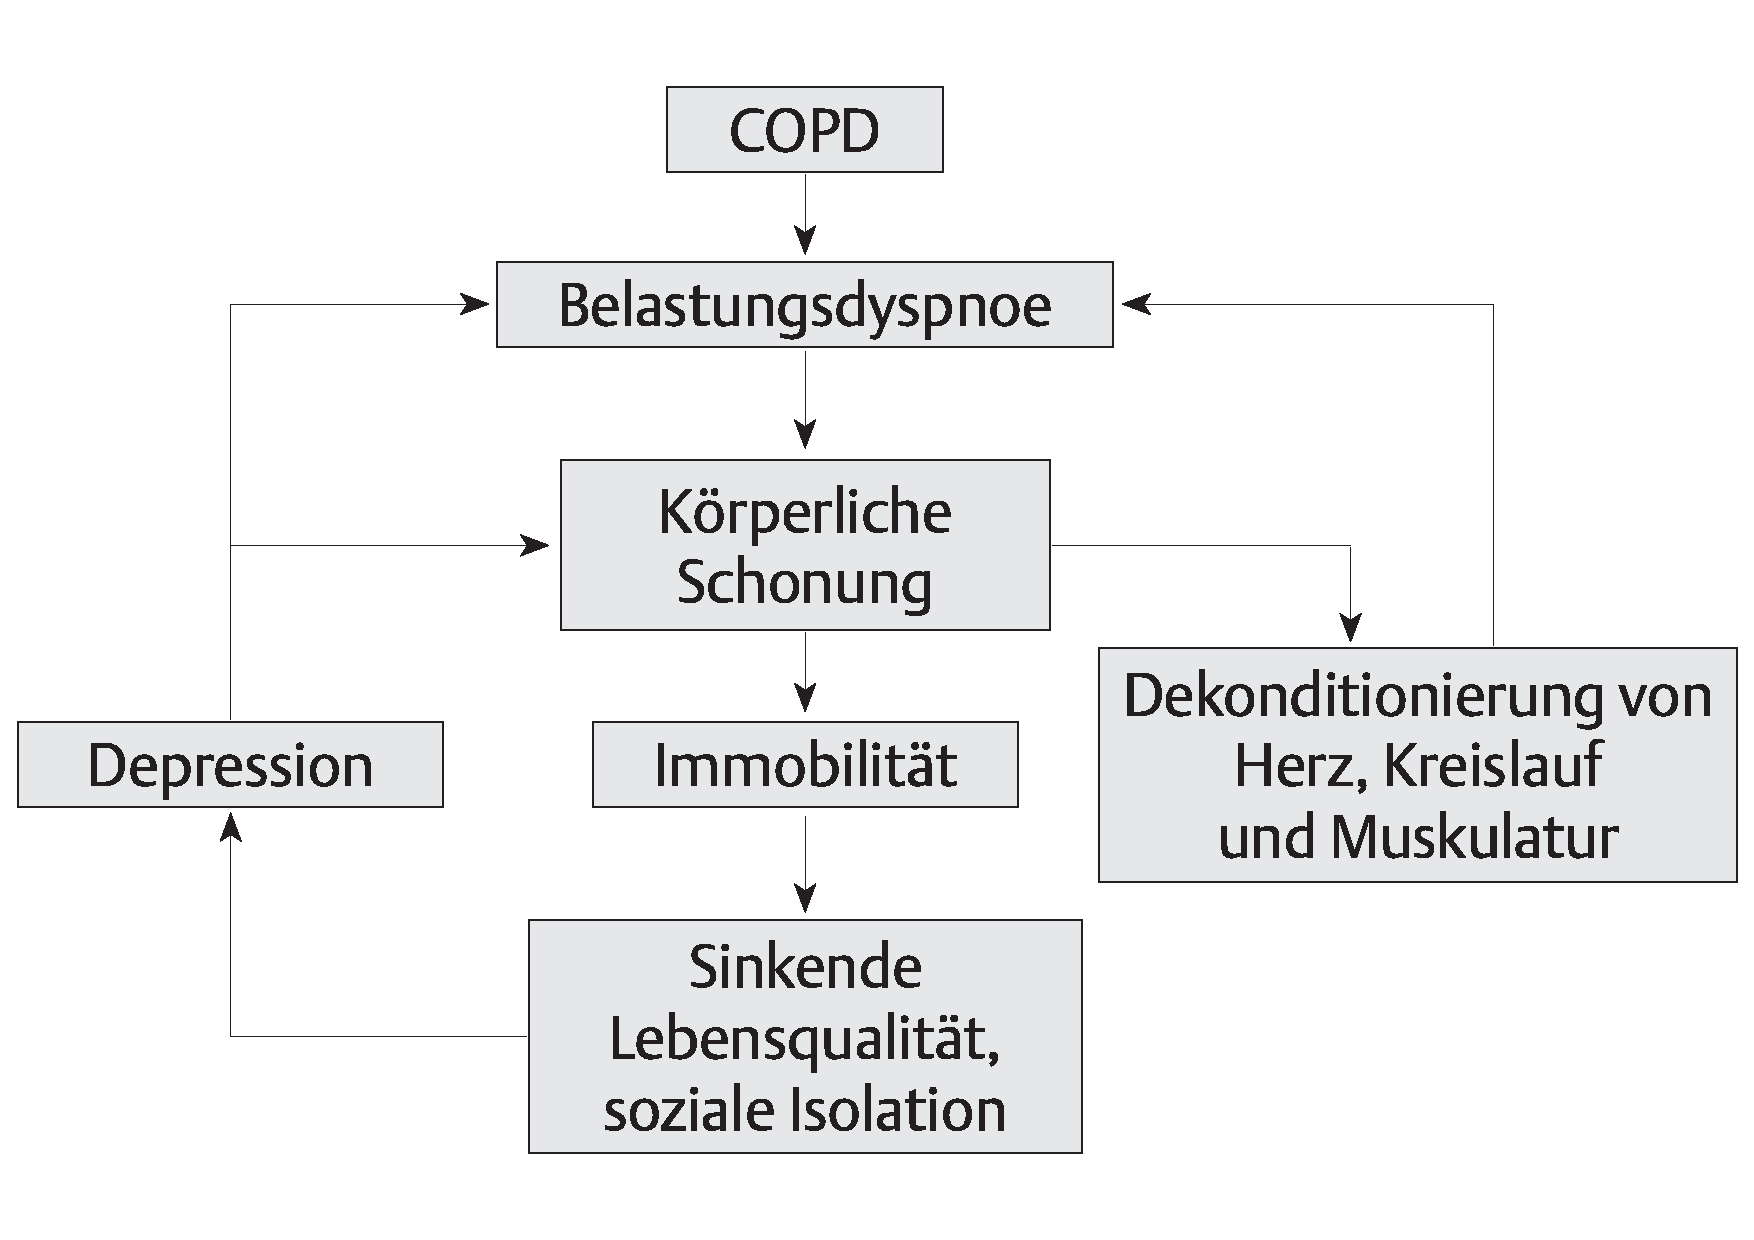
\includegraphics[width=0.6\textwidth]{teufelskreis}
  \caption{Circulus virtuosus, übernommen aus \cite[e19]{vogelmeier2007}}
  \label{fig:copd_teufelskreis}
\end{figure}

Die Angaben zur Prävalenz von Angst und Depression bei COPD variieren sehr. „Generalisierte Angststörungen werden in einer Häufigkeit von 2-16\%, Panikstörungen von 8-67\%, depressive Symptome und Depressionen zwischen 11 und 80\% sowie Angstsymptome in einem Bereich von 10-75\% angegeben“  \autocite[34]{kenn2011}.

An diesen Zahlen lässt sich erkennen, dass exakte Ergebnisse in Bezug auf die Prävalenz noch fehlen. Kenn und Kühl gehen davon aus, dass hierfür verschiedene methodische Diagnoseansätze verantwortlich sind. Generell erschwerte wohl neben den unterschiedlichen Erhebungsinstrumenten, wie Interviews und Fragebögen, auch die Heterogenität der untersuchten Patientenkohorte mit verschiedenen Schweregraden die Interpretation der Ergebnisse \autocite[vgl.][35]{kenn2011}.
Zudem geben die Studienergebnisse keine Auskunft darüber, in wieweit bei Patienten, die eine COPD aufgrund eines längeren Nikotinabusus entwickelt haben, bereits eine größere psychische Vulnerabilität und somit ein erhöhtes Risiko für die Ausbildung einer Depression oder Angst-/Panikstörung besteht. 

Ein evtl. wichtiges Konzept für den Krankheitsverlauf der COPD in seinen unterschiedlichen Facetten scheint die so genannten "`Fear Avoidance"' zu sein. Viele Patienten berichten von Angst vor auftretender Atemnot. Fear Avoidance- Konzept meint "`die Angst vor der Verstärkung eines Krankheitssymptoms bzw. Verschlechterung des Verlaufs und daraus folgende Aktivitätsvermeidung"' \autocite[111]{stenzel2013}. Dieses Konzept wurde jedoch bisher für COPD noch kaum diskutiert und erforscht. Eine neuere Studie zeigte jedoch, dass Fear Avoidance tatsächlich als Mediator des Zusammenhangs zwischen COPD-Status und Lebensqualität bzw. Gesundheitsstatus gesehen werden kann. Die Autoren plädieren daher dafür, dass im Rahmen der pneumologischen Rehabilitation auch psychotherapeutische Interventionen implementiert werden sollten, welche diesen Aspekt aufgreifen \autocite[vgl.][112]{stenzel2013}. 

In dem später dargestellten musiktherapeutischen Konzept wird dieser Aspekt ebenfalls implizit aufgenommen. Durch achtsames Wahrnehmen eigener Grenzen und Mög"-lichkeiten, aber auch übungszentriertes Arbeiten entwickeln die Patienten mithilfe positiver Erfahrungen im Zusammenhang mit Selbstregulation wieder mehr Selbstvertrauen und erleben sich als selbstwirksame Individuen, die sich nicht der auftretenden Atemnot ausgeliefert fühlen müssen.

In Studien wurde zudem ein signifikanter Zusammenhang zwischen einer erhöhten Mortalität und einer COPD mit begleitender depressiver oder Angstsymptomatik nachgewiesen. Aber auch in Bezug auf die Exazerbations- und Rehospitalisationsrate sowie die Leistungsfähigkeit und -bereitschaft von COPD-Patienten scheint hier die Ausbildung der genannten psychischen Erkrankung einen relevanten negativen Faktor darzustellen \autocite[vgl.][]{kenn2011}.

Obgleich das zuvor Erläuterte heutzutage unter allgemeinmedizinischen und pneumologischen Fachärzten als bekannt anzunehmen ist, wird die Problematik in den Arzt-Patienten-Gesprächen oftmals nicht thematisiert. Eine amerikanische Studie zeigte diese Diskrepanz zwischen der Prävalenz und Behandlungshäufigkeit psychischer Erkrankungen bei gleichzeitiger COPD. In einer Telefonumfrage von 1334 Patienten lagen bei 61\% psychische Auffälligkeiten, insbesondere Angstsymptome, vor. Lediglich 31\% dieser Patienten wurden diesbezüglich behandelt \autocite[vgl.][156]{fischer2007}.


\section{Zusammenfassende Betrachtung}
\label{zusammenfassende betrachtung}
Die vorherigen Ausführungen machen deutlich, um welch komplexes und schwerwiegendes Krankheitsbild es sich bei der COPD handelt. 
Durch Gespräche mit praktizierenden Lungenfachärzten und Betroffenen sowie durch Aussagen in unterschiedlichen Fachartikeln zeichnete sich für mich der Bedarf an psychologischer respensive psychotherapeutischer Begleitung sehr stark ab. Selbst in der pneumologischen Rehabilitation stellen Gespräche mit einem Psychologen ein freiwilliges Angebot dar. Aufgrund der meist starken Unterbesetzung an psychosozialem Fachpersonal ist die Versorgung hier meines Erachtens nur mangelhaft gegeben. Patienten, die sich eher in sich zurückziehen und wenig Eigeninitiative zeigen, haben so vermutlich nur geringe Chancen, eine Begleitung ihrer Bedürfnisse entsprechend zu erhalten. An dieser Stelle soll wie unter Kapitel \ref{section:gedanken_zum_setting} das in dieser Arbeit entwickelte musiktherapeutische Konzept greifen. Bevor jedoch auf dieses näher eingegangen wird, gibt das nächste Kapitel einen umfangreichen Einblick in das Thema "`Musiktherapeutische Stimmarbeit"' als solche.

% ---------------------------------------------------------------------------
% ----------------------- end of thesis sub-document ------------------------
\newpage\thispagestyle{empty}
% this file is called up by thesis.tex
% content in this file will be fed into the main document

%: ----------------------- introduction file header -----------------------
\chapter{Musiktherapeutische Stimmarbeit}
\label{chapter:musiktherapeutische_stimmarbeit}
\setlength{\epigraphwidth}{8.0cm}
\epigraph{Success depends upon previous preparation, and without such preparation there is sure to be failure.}{Confucius}
\ifpdf
    \graphicspath{{3_musiktherapeutische_stimmarbeit/figures/PNG/}{3_musiktherapeutische_stimmarbeit/figures/PDF/}{3_musiktherapeutische_stimmarbeit/figures/}}
\else
    \graphicspath{{3_musiktherapeutische_stimmarbeit/figures/EPS/}{3_musiktherapeutische_stimmarbeit/figures/}}
\fi
% ----------------------------------------------------------------------
%: ----------------------- introduction content -----------------------
% ----------------------------------------------------------------------
\lettrine{I}{n} this chapter, we introduce 


Herr \autocite[vgl.][12]{wolf2012} sagt, singen ist schön \autocite[9]{wolf2012}.
...them with 10Hz GNSS PVT\footnote{position, velocity, time} solutions. Because the MEMS-grade IMU exhibits a drift of more tha


\section{Einsatz der Singstimme in der Musiktherapie}
Bevor auf das Singen in der MT im Speziellen eingegangen wird, sollte der Blick auf den Gebrauch der Singstimme in der Gesellschaft gewendet werden, um ein klareres Gesamtbild dieses Themas entstehen lassen zu können.

Während das Singen, man beachte unseren großen Umfang an deutschem Liedgut, in unserer Großelterngeneration noch weit verbreitet war, so hat die nationalsozialistisch geprägte Zeit der 30er und 40er Jahre einen Keil in diesen selbstverständlichen Gebrauch der Singstimme in Gemeinschaft getrieben.
Die Verschandelung deutschen Liedguts mit nationalsozialistischem Gedankengut und den Einsatz desgleichen für propagandistische Zwecke sowie im Besonderen in der Jugendmusikbewegung der damaligen Zeit führte u.a. zu "der späteren Voreingenommenheit gegenüber gemeinsamem Singen im Allgemeinen und gegenüber dem deutschen Volkslied im Speziellen" \autocite[9]{wolf2012}.

Hinzu kommt die Entwicklung neuer Medien und die Möglichkeit eines geöffneten Zugangs zu diesen. Laut Wolf hat dies großen Einfluss auf "die Entwicklung hin zu einer Vereinzelung der Menschen und hin zu einer Veränderung des menschlichen Alltagverhaltens" \autocite[10]{wolf2012}, wodurch die Notwendigkeit der gemeinschaftlichen Freizeitgestaltung, welche in früheren Zeiten oftmals das gemeinsame Singen beinhaltete, nachließ. Nur an vereinzelten Schauplätzen wie z.B. im Gottesdienst, im Stadion, bei den Pfadfindern oder in Chören wird das gemeinschaftliche Singen und/oder Grölen noch aktiv praktiziert.

In der MT war der Einsatz der Singstimme ebenfalls lange Zeit negativ konnotiert und wurde "[\ldots] als "Konflikt vermeidende Technik" in den heilpädagogisch orientierten Bereich der Kindermusiktherapie oder das palliativ orientierte Feld der Geriatrie verortet" \autocite[10]{wolf2012}. So war das Singen von Liedern im Rahmen einer "psychotherapeutisch orientierten MT" lange Zeit ausgeklammert. Zudem wurde die Stimme zum klanglichen Ausdruck kaum genutzt, da man einen zu großen Widerstand seitens der Patienten erwartete. 

%Todo: Widerstand und Stimmeinsatz

Durch den sich in den letzten Jahren vollziehenden Paradigmenwechsel in der psychotherapeutischen Behandlung im Allgemeinen und der musiktherapeutischen im Speziellen von einem eher konfliktzentrierten Ansatz und dem Konzept der Katharsis hin zu einem eher ressourcenorientierten und stabilisierenden Arbeiten veränderte sich auch die Einstellung gegenüber dem Singen. Einer kleinen Forschergruppe aus Musiktherapeuten und -pädagogen, aber auch bekannten Ärzten (wie z.B. Dr. Gerald Hüther, Dr. Manfred Spitzer u.a.) ist es zu verdanken, dass wir heute mehr über die Wirkung des Singens auf Körper, Geist und Seele wissen. Sie waren es, die zu einer Etablierung von Singgruppenarbeit primär beigetragen haben. Im klinischen Bereich hat sich insbesondere Wolfgang Bossinger verdient gemacht und eine mittlerweile über Deutschland verbreitete Initiative, "Singende Krankenhäuser", ins Leben gerufen. Aber auch Sabine Rittner und Karl Adamek haben zu einem großen Erkenntnisgewinn und möglichen Vorgehensweisen in diesem Bereich verholfen.

Heute wird die (Sing-)Stimme im psychotherapeutischen Kontext in unterschiedlicher Art und Weise eingesetzt, genutzt und betrachtet. Sabine Rittner todo hat diese Bereiche kategorisiert, um ihre Komplexität zu entzerren. Diese insgesamt acht Kategorien fließen in die folgenden Ausführungen ein: 
Stimme als\ldots
\begin{enumerate}
\item Medium der verbalen und nonverbalen Beziehungsgestaltung
\item Methode in der körperorientierten Musikpsychotherapie
\item Diagnostikum im therapeutischen Gespräch
\item Indikator für die therapeutische Übertragung- und Gegenübertragung
\item Symptom
\item Ausdrucksmittel
\item Selbstheilungs-Mittel
\item Medium zur Tranceinduktion
\end{enumerate}
Im Rahmen der Diagnostik gibt die Stimme des Patienten bereits wichtige Hinweise auf dessen aktuelle Befindlichkeit, seine Stimmung und durch aufmerksames Hinhören kann erspürt werden, ob das Gesagte in sich "stimmig", sprich kongruent ist. Zudem gibt sie bereits Auskunft über den biografischen Hintergrund der sich äußernden Person, denn sie hat sich mit unseren über die Zeit gesammelten Lebenserfahrungen weiterentwickelt und diese in sich aufgesogen. So gilt die Stimme unter Experten als "Klingendes Hologramm der Persönlichkeit" \autocite{adamek1999} "lauthafte Biographie" \autocite{gundermann1994} und bei Rittner erfahren wir über den Klang der Stimme etwas über die "leib-seelische Gewordenheit" \autocite[211]{rittner2008} des Menschen.
Dabei scheint jedoch nicht so sehr der Inhalt des Gesagten aufschlussreich, sondern vielmehr der "Klang der Stimme (Klangspektrum, Modulation, Lautstärkeänderungen, Stimmsitz, Vokaleinsatz etc.), die Sprechweise (Artikulation, Phrasierung, Pausensetzung etc.) und die Atmung (Atemfrequenz, Atemtiefe, hörbares Einatmen, Sitz des Atemraumes im Körper etc.)" als auch "die Art der Gestaltung von Sprechpausen, Abbrüchen, Momenten des Innehaltens, Verzögerungen u.ä." \autocite[210]{rittner2008}. Diese stillen Momente, wie


Die Wirkung des Singens auf Körper und Psyche
Bossinger, Adamek und Cramer

Wirkungsfähigkeiten des Singens im therapeutischen Kontext

Die Rolle der Stimme für die Diagnostik




\newpage\thispagestyle{empty}
% ----------------------------------------------------------------------
% this file is called up by thesis.tex
% content in this file will be fed into the main document

\ifpdf
\graphicspath{{4_konzept/figures/PNG/}{4_konzept/figures/PDF/}{4_konzept/figures/}}
\else
    \graphicspath{{4_konzept/figures/EPS/}{4_konzept/figures/}}
\fi

%: ----------------------- introduction file header -----------------------
\chapter{Konzeptionelle Ueberlegungen}
\label{chapter:konzeptionelle_ueberlegungen}
Die vorangegangenen Auseinandersetzungen mit den Themen COPD und Musiktherapeutische Stimmarbeit dienten dem Aufbau einer Basis, um nun auf dieser ein eigenes Konzept entwickeln zu können. 

Dieses Konzept für die musiktherapeutische Stimmarbeit mit COPD-Patienten ist als übungs- und erlebniszentriertes sowie ressourcenorientiertes Gruppenverfahren angelegt, welches auf der Grundlage psychodynamisch orientierter Musiktherapie Aspekte aus der Körper- und Atemarbeit, Achtsamkeitslenkung und Gesangspädagogik mit einbezieht. Die folgenden Abschnitte sollen dies nun weiter ausführen und erklären. Am Ende des Kapitels wird ein beispielhafter Sitzungsaufbau beschrieben. Um für die Praxis gut vorbereitet zu sein, wurden im Verlauf des Masterarbeits-Prozesses verschiedene Übungen gesammelt, welche jedoch aus Platzgründen zum Teil dem Anhang zum interessierten Nachlesen beigefügt wurden.


\section{Psychodynamische Überlegungen}
\label{psychodynamische ueberlegungen}
In \ref{copd} wurde bereits dargelegt, dass die Diagnose einer COPD auch auf psychischer Ebene für Patienten mit Veränderungen verbunden sein kann. In welchem Ausmaß dies geschieht und mit welchen Folgen es verbunden sein kann, ist sehr individuell verschieden und hängt mit den jeweiligen biographischen Hintergründen und den damit verbundenen Entwicklungsmöglichkeiten hinsichtlich einer stabilen, gefestigten psychischen Verfassung sowie mit einem unterstützenden sozialen Umfeld zusammen. 
Wie bereits unter 2. näher erläutert, wird eine COPD nur unter bestimmten Umständen ausgebildet: genetische Veranlagung (ein sehr verschwindend geringer Teil), Umweltverschmutzung und Einatmen von Schadstoffen bspw. im beruflichen Umfeld sowie zum größten Teil durch einen länger andauernden Nikotin-Abusus (betrifft ca. 80\% der Patienten). 

Was bedeutet aber letzteres nun für die therapeutische Behandlung dieser Patienten? M.E. scheint es wichtig diesen Aspekt mitzudenken und aufzugreifen, da damit oftmals  suchtspezifische psychische Aspekte verbunden sind und diese Besonderheiten insbesondere in der Gegenübertragung mit sich bringen und somit für die Behandlung abhängiger Patienten die Auseinandersetzung mit diesem Thema seitens des Therapeuten unumgänglich erscheint. Es ist mir natürlich bewusst, dass mit dieser Erklärung nicht alle potentiellen Patienten eingeschlossen sein werden, aber aufgrund der hohen Relevanz der Nikotinabhängigkeit in Verbindung mit der Ausbildung einer COPD bedarf es eines Einbezugs dieser Problematik in therapeutische Konzepte. Es gilt natürlich in der Praxis diese Annahmen stets zu überprüfen und bei Bedarf anzupassen bzw. individuell zu verändern. 

Bevor jedoch auf spezielle psychodynamische Aspekte eingegangen wird, bedarf es einer kurzen definitorischen Erläuterung, was unter dem Phänomen Sucht im deskriptiven Sinne verstanden werden kann. 
\begin{quote}
\emph{"Das süchtige Verhalten besteht in dem anhaltenden, starken, unwiderstehlichen Drang, bestimmt durch Drogen bzw. andere Substanzen oder auch durch Tätigkeiten [...] hervorgerufene innere Zustände und Befindlichkeiten von Entspannung oder Anregung immer wieder aufzusuchen oder herbeizuführen."} \autocite[173]{mentzos2011} 
\end{quote}
Betroffene tendieren dazu, im Verlauf die Suchtmittel-Dosis immer mehr zu erhöhen. So seien die Übergänge zwischen normalem Gebrauch und Missbrauch des Suchtmittels bis zur psychischen und körperlichen Abhängigkeit fließend \autocite[vgl.][173]{mentzos2011}. Im ICD-10 findet sich das Störungsbild der Tabakabhängigkeit unter F17 im Bereich der psychischen Störungen; auch das DSM-IV beschreibt das Störungsbild in ihrem Diagnostischen und Statistischen Manual Psychischer Störungen. Um eine Abhängigkeit diagnostizieren zu können, müssen mindestens drei von insgesamt sechs im ICD-10 beschriebenen Kriterien seit 12 Monaten vorherrschen. Diese umfassen:

\begin{itemize}
\item "starkes Verlangen oder eine Art Zwang, Substanzen oder Alkohol zu konsumieren
\item verminderte Kontrollfähigkeit
\item körperliches Entzugssyndrom
\item Toleranzentwicklung (Dosissteigerung)
\item Vernachlässigung anderer Interessen
\item anhaltender Substanz- oder Alkoholkonsum trotz Nachweis schädlicher Folgen (körperlich, psychisch sozial)" \autocite[315]{moeller2009}
\end{itemize}

Für die Entstehung und Aufrechterhaltung der Sucht dürfen natürlich die neurobiologischen Prozesse nicht außer Acht gelassen werden. Es wird davon ausgegangen, dass "es sich bei der stoffgebundenen Sucht um die neurochemische Anpassung des Gehirns an eine anhaltende Substanzzufuhr" \autocite[14]{tretter2008} handelt. Den Antrieb für das süchtige Verhalten bilde hiernach ein neurochemisch begründbarer Belohnungseffekt des Suchtstoffes. Dieser Aspekt ist m.E. selbst aus psychodynamischer Sicht wichtig, da es hier vermutlich zu einem Wechselspiel unterschiedlicher Faktoren kommt und sich aus einer vormals psychischen Abhängigkeit oftmals eine körperliche entwickeln kann.
Darüber hinaus bestehen in Bezug auf die Hintergründe der Suchtentwicklung noch weitere theoretische Modelle (Verhaltenstherapie, Stress-Konzept u.a.) \autocite[vgl.][38ff.]{tretter2008}, auf welche jedoch an dieser Stelle nicht weiter eingegangen werden kann.
 
Folgt man psychoanalytischen Theorien zur Suchtentwicklung, kann davon ausgegangen werden, dass bei Menschen mit einer ausgeprägten Suchtproblematik in der frühen Kindheit ein wichtiger Erfahrungsbereich nicht ausreichend genährt wurde: ein Gefühl eigener Bedürfnisse ist nicht ausreichend entwickelt sowie die Wichtigkeit des sich dafür Einsetzens erkennen und eigenverantwortlich umsetzen zu können. Dafür bedarf es der frühen Erfahrung, dass ein Kind im Außen diese auf sich bezogene und abgestimmte Zuwendung und Wertschätzung erfahren hat. Austauschprozesse zwischen dem Kind (dem Selbst) und dem Anderen (dem Objekt) im zuvor genannten Sinne, wodurch das heranwachsende Kind "gute" Objekte internalisieren kann, sind essentiell für die Entwicklung einer stabilen Persönlichkeit. Dieses Postulat entspringt primär der Objektbeziehungstheorie. In Bezug auf die Suchterkrankung wird hier davon ausgegangen, dass es sich immer um eine Beziehungskrankheit handelt, welche vermutlich ihren Ursprung in der frühen Kindheit im Übergang von der Symbiose zur Individuation hat \autocite[vgl.][9]{weidlinger2012}. Kann das Kind aufgrund wiederholter Ablehnung, mangelhafter Feinfühligkeit oder gar wegen an ihm ausgeübter körperlicher oder seelischer Gewalt kaum positive Selbstobjekte ausbilden, so werden an deren Stelle negative Selbstobjekte treten und das Kind wird vermutlich im weiteren Verlauf innerlich mit ambivalenten, polarisierenden Gefühlen sowie mit der Schonung oder aggressiver Wut auf die Objekte beschäftigt sein\autocite[vgl.][10]{weidlinger2012}. 

Diese Ambivalenz zeigt sich ebenfalls in der Sucht, da das Suchtmittel als Beziehungsobjekt sehr ambivalent besetzt ist. "Auf der einen Seite wirkt es tröstend, beruhigend, entängstigend oder berauschend und anregend; auf der anderen Seite aber bringt es dem Süchtigen Leid, Schuldgefühle, körperliche und seelische Zerstörung bis hin zum Tod" \autocite[175]{mentzos2011}. Jedoch zeigt sich hierin m.E. primär die "verinnerlichte Tendenz zur Selbstabwertung wie Selbstzerstörung" \autocite[10]{weidlinger2012}. Diesen Aspekt, des mangelnden Selbstwertgefühls aufgrund einer strukturellen Störung, findet sich in den psychodynamischen Theorien der Sucht immer wieder an. 

Beispielsweise in der Sucht-Theorie der Selbst-Psychologie nach Kohut, wird dem Suchtmittelkonsum die Funktion einer Ersatzbefriedigung hinsichtlich mangelhaft genährter narzisstischer Bedürfnisse zugeordnet. Auch Mentzos (2011) schreibt, dass "das Suchtmittel(...) zum Mittel der notdürftigen Kompensation einer gestörten Selbstwertgefühlregulation" werde, das heißt als Ersatz für ein stützendes narzisstisches Selbstobjekt dient. So kann das Suchtverhalten auch als Versuch des Betroffenen verstanden werden, die eigene, innere Sicherheit mithilfe des Suchtmittels wieder herzustellen, welche zuvor durch Enttäuschungen, Kränkungen, Vernachlässigung oder tiefgreifende Konflikte verloren gegangen war. Tress zufolge handelt es sich bei der Sucht um einen Versuch der "Selbstheilung"(\cite{tress1985} zitiert in \cite[222]{ermann1999})

Folgt man diesen vorherigen Überlegungen, so kann davon ausgegangen werden, dass bei Menschen mit einer entwickelten Suchtproblematik eine erhöhte Vulnerabilität in Bezug auf ihr Selbstempfinden besteht. Dieser Aspekt könnte meines Erachtens in Bezug auf die Krankheitsbewältigung einer ausgebildeten COPD wichtig sein, wie im Folgenden näher erläutert wird.

Bei Daniel Stern finden sich sehr essentielle Vorstellungen für die Entwicklung eines Selbstempfindens wieder. Diese sind jedoch nicht nur in Bezug auf die kindliche Entwicklung von großer Wichtigkeit, sondern bleiben es für das gesamte Leben. Stern unterscheidet hierbei zwischen sechs verschiedenen Bereichen, welche letztlich das Selbst des Menschen bilden: das auftauchende Selbst, das Kern-Selbst, das intersubjektive Selbst, das verbale Selbst sowie mittlerweile das narrative Selbst. Dabei gliedert er seit ein paar Jahren die Empfindung eines Kern-Selbst in zwei Bereiche: zum Einen in die Empfindung eines Kern-Selbst mit seinen drei Invarianzen von Urheberschaft, Kohärenz und Kontinuität und zum Anderen in die Empfindung eines Kern-Selbst in Gemeinschaft mit dem Anderen.  Wie in der Grafik ersichtlich wird, haben die ersten 3 Bereiche nach Sterns neueren Erkenntnissen ihren Ursprung bereits in der pränatalen Phase.


\begin{figure}
 \centering
  \includegraphics[width=0.7\textwidth]{selbstempfindungen}
  \caption{Die sechs Selbstempfindungen nach Daniel Stern}
  \label{fig:selbstempfindungen}
\end{figure}

Da an dieser Stelle nicht auf alle Bereiche des Selbstempfindens ausführlich eingegangen werden kann, empfiehlt sich ein Blick in Daniel Sterns Werk "Die Lebenserfahrung des Säuglings", in welchem der Entwicklungspsychologe, Säuglingsforscher und Psychoanalytiker in sehr anschaulicher Weise die Entwicklung des Säuglings anhand der Entwicklung eines umfassenden Selbstempfindens erläutert.

In Bezug auf eine entwickelte COPD scheint es naheliegend, sich mit der Entwicklung eines Kern-Selbst und hier insbesondere mit der Invarianz der Urheberschaft zu beschäftigen, wobei nicht außer Acht gelassen werden darf, dass alle Bereiche ineinander greifen und sie letztlich nur theoretisch auseinanderdividiert werden können.

Nun aber warum scheint eine besondere Auseinandersetzung mit der o.g. Invarianz in Bezug auf eine COPD sinnvoll?!

Das Empfinden eines Kern-Selbst entsteht aus dem Zusammenspiel der zuvor genannten Invarianzen der Selbsterfahrung, d.h. unveränderlicher Erfahrungsmuster, die zu einer Organisation und Struktur innerer Prozesse führen. Wie aus der Grafik hervorgeht, handelt es sich um Entwicklungsbereiche, die sich hier natürlich auf den Lebensanfang beziehen, jedoch die Grundlage jeglicher Selbstempfindung bilden. So können sich die einzelnen Bereiche immer weiter ausdifferenzieren, die Basis jedoch bleibt bestehen. 
Stern beschreibt das "Kern-Selbst-Empfinden […] (als) ein erfahrungsgeleitetes Empfinden von Vorgängen, das wir normalerweise als völlig selbstverständlich voraussetzen und uns nicht bewusst machen. […] Das Selbstempfinden ist kein kognitives Konstrukt; es ist die Integration des Erlebens.“ \autocite[106f.]{stern2007} Er bezeichnet es sogar als "die Grundlage für alle differenzierten Selbstempfindungen, die sich später entwickeln werden“ \autocite[106f.]{stern2007}. 

Was passiert jedoch, wenn ein Mensch spürt, dass er zuvor selbstverständliche körperliche Prozesse, wie im Fall der COPD die Atmung, nicht mehr so steuern kann, wie er möchte? Dies spricht m.E. in erster Linie die Invarianz der Urheberschaft an. Sie umfasst das Empfinden, Urheber eigener Handlungen zu sein als auch Nicht-Urheber der Handlungen anderer. Dies ist stets verbunden mit einem willentlichen Vorgehen, der propriozeptiven Wahrnehmung als auch dem Wissen, dass dieses Vorgehen bestimmte Konsequenzen nach sich zieht \autocite[vgl.][106, 114f.]{stern2007}. Im Falle der pneumologischen Veränderungen bei einer COPD, welche stets einhergehen mit ansteigender Atemnot scheint dieses Gefüge nun ins Wanken zu kommen: die Atmung als "selbstverständlicher" und meist nicht bewusst gesteuerter Vorgang verändert sich und dem COPD-Patienten scheint die Kontrolle über diesen Vorgang in manchen Situationen zu entgleiten. Dabei gerät jedoch primär der erste Teil dieser Invarianz, das willentliche Vorgehen, in eine unsichere Position, während die propriozeptive und im Falle der COPD auch die viszerozeptive Wahrnehmung intakt ist und eine Konsequenz für diese körperlichen Vorgänge erahnt werden kann. Dies kann verständlicherweise zu Unsicherheit führen. Bei Menschen, die über ein stark ausgebildetes Ich, ein haltendes und unterstützendes soziales Umfeld sowie über ausreichende Copingstrategien verfügen, wird der Bedarf an professioneller therapeutischer Begleitung vermutlich nicht so hoch sein, wie bei oben beschriebenem Klientel, welches aufgrund einer frühen mangelnden bzw. adäquaten Zuwendung nicht über die genannten Ressourcen verfügen. 

Wiederholt sich dieser Vorgang stetig, kann es zu einer Schwächung regulierender Selbstobjekte führen, welche bereits im Säuglingsalter durch die Interaktion mit einem selbstregulierenden Anderen beginnen, sich herauszubilden \autocite[vgl.][338f.]{stern2007}. Je nach individueller Ausprägung der regulierenden Selbstobjekte kann dieser Vorgang früher oder später in eine Regression des Patienten münden. Nun wird die Regulierung auftauchender affektiver Zustände im Außen wieder wichtiger. 
An dieser Stelle kann an eine frühe Erfahrungswelt im Rahmen eines therapeutischen Settings angeknüpft werden, wenn ein geschützter, haltender, stützender und/oder nährender Rahmen geschaffen werden kann \autocite[vgl.][58ff.]{timmermann2008}. Insbesondere die Arbeit mit der Stimme eignet sich hier besonders. Da die Stimme der primären Bezugspersonen am Anfang des Lebens i.d.R. verbunden wird mit der Erfahrung eines geschützten, nährenden Raums, "werden wir [lebenslang] in den Tiefen unseres Unbewussten mit Stimmausdruck eine >heile Welt< assoziieren" \autocite[282]{deckervoigt2000}. Das "heil" bezieht Decker-Voigt in diesem Zusammenhang darauf, dass uns der Klang der Stimme an eine Zeit erinnere, in der wir Kränkungen, Beängstigungen und Verletzungen seelisch noch ertragen konnten \autocite[vgl.][282]{deckervoigt2000}. 

Darüber hinaus scheint in Bezug auf eine angstfreie Ausbildung eines Kern-Selbst auch ein sicherer, haltender Rahmen notwendig. Greift man zurück auf die Erfahrungen des Säuglings, so wissen wir, dass die Entwicklung stets gekoppelt ist an die Verfügbarkeit der primären Bezugspersonen und ihrem Umgang mit dem Säugling. Für eine gelingende Entwicklung ist es wichtig, dass die primären Bezugspersonen (i.d.R. Mutter und Vater) feinfühlig auf das Kind eingehen und als sichere emotionale Basis für das Kind verfügbar sind (Begriffe aus der Bindungstheorie nach J. Bowlby und M. Ainsworth, siehe \cite{brisch2013}) sowie durch Synchronisationsprozesse mit dem Säugling zur Ausbildung einer stabilen psychischen Struktur beitragen. Da zu Beginn des Lebens noch nicht die Möglichkeit zur Selbstregulation gegeben ist, sind auch für diesen Funktionsbereich die primären Bezugspersonen von großer Wichtigkeit. Wird der Säugling allein gelassen mit dieser Überstimulierung durch unbekannte Reize und kann sein eigenes Gefühlschaos nicht selbst regulieren, wird er sich vermutlich ängstlich zurückziehen. Hat er jedoch im Außen ein (markiert) spiegelndes \autocite[vgl.][153]{fonagy2004}, feinfühliges Gegenüber, so kann er nach und nach diese nun sich ausbildenden Repräsentanzen in seine psychische Struktur integrieren. 
Übertragen auf die Situation eines erwachsenen Menschen mit COPD kann dies bedeuten, dass er für die Bewältigung seiner gesundheitlichen Krise und zur Prävention vor komorbiden psychischen Störungen von einem regulierenden Anderen profitieren würde. Häufig jedoch sind die näheren Angehörigen aufgrund eigener Involviertheit nicht in der Lage, diesen stützenden Part zu übernehmen oder die Beziehung ist aufgrund der Krankheitssituation bereits zu sehr belastet. 

Daher kann es hilfreich sein, außerhalb der gewohnten sozialen Bezüge einen Raum für sich in Anspruch nehmen zu können, in dem es um die eigene Person geht, so wie sich zu Beginn des Lebens in einem geschützten Rahmen die Handlungen der Bezugspersonen am Säugling orientieren. Im Rahmen einer tiefenpsychologisch fundierten Musiktherapie, wie sie in dieser Arbeit vertreten wird, steht stets der "Musik erlebende und sich durch Musik ausdrückende Mensch als Klient" im "Zentrum der Aufmerksamkeit" \autocite[4]{timmermann2004}. Für den Umgang mit der Erkrankung bringt jeder vor dem Hintergrund seiner individuellen Kindheitsgeschichte Copingstrategien und Ressourcen mit, die ihm helfen, die Situation, zu bewerkstelligen. In manchen Fällen ist es jedoch sinnvoll, sich dieser gewahr zu werden, zu verstehen, wie und aus welcher Situation diese entstanden sind und neue Wege auszuprobieren. 

\section{Therapeutische Grundhaltung} 
Wie im vorherigen Kapitel ersichtlich, bildet das psychoanalytisch-tiefenpsychologische Verständnis von seelischen Prozessen sowie entwicklungspsychologisches Wissen die Grundlage meiner Arbeit. Meine Grundhaltung ist jedoch mit den Jahren durch die Auseinandersetzung mit anderen Schulen (u.a. während meines Sozialpädagogikstudiums) gewachsen und beinhaltet daher Schulen-übergreifende Aspekte. 

Für die therapeutische Arbeit erachte ich den Aufbau einer haltenden, vertrauensvollen Beziehung, welche von Respekt und Achtsamkeit geprägt ist, als wesentlich. 
Im Rahmen dieser ist es die Aufgabe des Therapeuten, empathisch und kongruent auf sein Gegenüber einzugehen, stets dessen Individualität und subjektive Wahrnehmung akzeptierend. 
Es geht für mich um Begleitungs- und Verstehensprozesse, welche die unterschiedlichen Ebenen der therapeutischen Arbeit, Übungs-, Erlebnis- und Konfliktzentrierung, je nach Kontext und Bedarf nutzt, um darüber hinaus mit dem Patienten angemessene Veränderungs- bzw. Weiterentwicklungsprozesse anzustoßen und voranzubringen. 

In der Arbeit mit COPD-Patienten scheint es m.E. sinnvoll, die Arbeit vorerst primär übungs- und erlebniszentriert sowie ressourcenorientiert auszurichten, da aufgrund begrenzter Zeit (siehe \ref{section:gedanken_zum_setting}) und vermutlicher Abwehr gegenüber einem psychotherapeutischen Verfahren im Hinblick auf die Therapieziele eine tiefere Bearbeitung bestehender Konflikte nicht sinnvoll erscheint. Nicht sinnvoll daher, weil ein weiteres Auffangen und Bearbeiten evtl. aufgrund des Settings (siehe \ref{section:gedanken_zum_setting}) nicht mehr möglich ist. Sollte es jedoch im Verlauf der Behandlung sinnvoll oder gar notwendig erscheinen, auf solche tiefer einzugehen, ist dies natürlich nicht ausgeschlossen. Allerdings ist es hier erforderlich, immer wieder zu hinterfragen, ob dies tatsächlich für den Patienten momentan tragbar oder evtl. sogar zu überfordernd ist. Insbesondere dann, wenn dies in der Gegenübertragung spürbar wird. Dieser Aspekt ist m.E. für die gesamte Behandlung wichtig, egal auf welcher Ebene gearbeitet wird. COPD-Betroffene sind meist primär mit ihrer Erkrankung beschäftigt und eine bewusste Aufarbeitung psychischer Konflikte könnte schnell destabilisierend wirken, da bereits der Prozess der Krankheitsbewältigung teilweise sehr kraftraubend wirkt. Zu dieser Einschätzung komme ich durch persönliche Gespräche und Erfahrungsberichte von Betroffenen, welche ich im Verlauf der Auseinandersetzung mit der Arbeit geführt oder gehört/ gelesen habe. 

Eventuell ergibt sich im Anschluss an eine rehabilitative Maßnahme aber eine längerfristige ambulante Therapie, welche wiederum neue Möglichkeiten eröffnet. 

Darüber hinaus scheint mir für die therapeutische Arbeit mit diesem Klientel, wie zuvor erläutert, der Sucht-Aspekt sehr wichtig. Ich vermute, dass sich in der Behandlung dieser Patienten diese Abhängigkeitsthematik auch in der Beziehung zum Therapeuten zeigen kann. So könnten einerseits die unbewussten Wünsche nach Ich-verstärkenden Reaktionen bzw. auch das Gegenteil wie oben beschrieben i.S. der Selbstzerstörung an den Therapeuten herangetragen werden. Hier gilt es in der Gegenübertragung sehr aufmerksam zu sein und diese Tendenzen nicht auszuagieren, sondern vielmehr Interventionen anzubieten, welche die Selbstwirksamkeit des Einzelnen stärkt und ihn auf sich zurückführt. Gerade bei Patienten mit einer körperlichen Erkrankung scheint mir hier die Aufmerksamkeitslenkung auf den Körper und die Atmung sehr hilfreich. Ohne gleich zu tief in psychische Themen einzusteigen, werden diese doch unumgänglich mit bearbeitet (siehe \ref{section:einbezug von koerper und atem}). 

\section{Therapieziele}
Hierin kann an die vorherigen Ausführungen gut angeschlossen werden. Eines der mir am wichtigsten erscheinenden Ziele ist die Steigerung der Selbstwirksamkeit. Dieser Gesichtspunkt knüpft sowohl an das Sternsche Thema der Urheberschaft als auch an den unter \ref{psychische_komorbiditaet} beschriebenen Circulus Virtuosus an. Die Erfahrung, das eigene Befinden selbst beeinflussen und verändern zu können, kann im Rahmen musiktherapeutischer Stimmarbeit, wie sie hier konzipiert ist, einen wesentlichen Beitrag zur Förderung dieses Bereiches bieten. Atemvertiefung, sensibilisierte Körperwahrnehmung, Singen als (evtl. wiederentdeckte) Ausdrucksform, die Einbindung in eine und der Austausch innerhalb einer Gruppe sowie positive Beziehungs- und Selbsterfahrungen im Rahmen der therapeutischen Beziehung sind m.E. weitere Aspekte, welche zur Stärkung dieses Bereiches beitragen können.

Mit Fortschreiten der Erkrankung nimmt in der Regel auch die (subjektive) Lebensqualität Betroffener immer mehr ab. Aus diesem Grund scheint es mir als eine wesentliche Aufgabe, die Steigerung der Lebensqualität auch als Ziel in dieses Konzept aufzunehmen. Ein wichtiges Ergebnis neuerer Singforschung, welche sich dem Thema "Singen und COPD" widmete (siehe \ref{copd_in_der_singforschung}, zeigte zudem, dass insbesondere die Lebensqualität Betroffener durch eine regelmäßige Teilnahme an einem Singangebot signifikant gesteigert werden konnte. 

Zudem konnte festgestellt werden, dass durch die Steigerung der Lebensqualität eine geringere Wahrscheinlichkeit zur pathologischen Ausbildung einer depressiven oder Angstsymptomatik bestand, was zudem einen Ausweg aus dem beschriebenen COPD-Teufelskreis bedeuten könnte. So enthält dieses Konzept auch die Absicht der Prävention bzgl. der sich oftmals im Verlauf der COPD zeigenden Komorbiditäten wie Depression und Angst.

Für einige mag gerade die akute Gesundheitsverschlechterung zum ersten als auch zum wiederholten Male zu einem krisenhaften Erleben der eigenen Situation führen. Dies kann durchaus auch mit der Auseinandersetzung der Begrenztheit des eigenen Lebens sowie mit dem bewussten Auftauchen der Todesangst einhergehen. Hier kann es das Ziel musiktherapeutischer Arbeit sein, Patienten einen Ort für die Wahrnehmung, Akzeptanz und den Umgang mit den damit verbundenen Affekten zu eröffnen und sie darin zu begleiten, die Möglichkeiten zum persönlichen Wachstum und zur Weiterentwicklung zu erkennen und zu nutzen, welche jeder Krise innewohnen. Dabei scheint es förderlich, durch den Austausch mit einem oder mehreren Spiel- und Gesprächspartnern und die bewusste Auseinandersetzung mit der bisherigen Selbsteinschätzung und Lebenssituation neue Sichtweisen auf sich und die eigene Lebensbehandlung zu entwickeln. Hier stellt die Musik und insbesondere der stimmliche Ausdruck eine wichtige Ergänzung zur Sprache dar, denn durch den Wechsel vom Darüber-Reden zum Es-Spielen kann ein sehr hilfreicher Ausweg aus den herkömmlichen Denk- und Fühlschablonen geschaffen werden. Hierin enthalten ist zudem das Thema der Krankheitsbewältigung, welches mir für die Arbeit mit diesem Klientel als sehr wesentlich erscheint. Aufgrund der mangelnden psychologischen Betreuung, häufiger sozialer Isolation mit Fortschreiten der Erkrankung sowie seltenem Kontakt zu anderen COPD-Patienten fehlen Betroffenen oftmals Austauschmöglichkeiten über krankheitsimmanente Themen und Fragen und verbleiben so in ihrer eigenen Gedanken- und Phantasiewelt. Hierfür scheint mir die Arbeit in der Gruppe sehr sinnvoll, wie im folgenden Kapitel näher erläutert werden soll.

\section{Gedanken zum Setting}
\label{section:gedanken_zum_setting}
Die vorangegangene Darstellung der therapeutischen Ziele deutet bereits darauf hin, dass in diesem Kontext die Arbeit in der Gruppe sinnvoll erscheint. Insbesondere Patienten, die von sozialer Isolation bedroht sind und Schwierigkeiten (entwickelt) haben, sich in sozialen Gruppen zu bewegen, können in einem geschützten und durch die Therapeutin gehaltenen Rahmen neue Erfahrungen sammeln, diese reflektieren und über diesen Prozess Vertrauen fassen in die eigenen Kontaktmöglichkeiten.

Zudem kann es im Austausch mit der Gruppe zur Hinterfragung der eigenen Lebens-be-handlung kommen und alternative Umgangsformen und Lösungsstrategien entwickelt werden. 

Vielen Patienten fehlt oftmals der Kontakt zu anderen Betroffenen und es fällt ihnen schwer, aus eigenem Antrieb sich an Selbsthilfegruppen oder Beratungsstellen zu wenden. Dies kann auch aus einem geschwächten Gefühl für eigene Bedürfnisse und eine verzerrte Selbstwahrnehmung resultieren. Auch hier kann der Einzelne gerade von der Gruppensituation profitieren, da hier ein Raum für den Abgleich von Selbst- und Fremdwahrnehmung geschaffen werden kann.

Gerade für die Krankheitsbewältigung kann der Austausch innerhalb einer diagnosespezifischen Gruppe daher hilfreich und unterstützend wirken. Um jedoch den oben entwickelten Gedanken in Bezug auf ein haltendes, stützendes und spiegelndes Gegenüber innerhalb eines geschützten Rahmens, in welchem ein Raum zum Ausprobieren, Reflexion, Stärkung und Veränderung geboten wird, gerecht zu werden, bedarf es einer therapeutisch ausgebildeten Leitung dieser Gruppe. 

Zudem scheint mir das Gruppensetting hinsichtlich der Suchtthematik als sinnvoll. Während in der Einzeltherapie die Ablösungsschritte vom Therapeuten zugunsten einer größeren Autonomie beschwerlicher sind, können diese durch die Sicherheit-gebende Gruppe leichter ausprobiert und gegangen werden \autocite[vgl.]{nawe2014}. Gerade in Bezug auf die Stärkung der Selbstwirksamkeit ist dies meines Erachtens ein wichtiger Aspekt.

Um diesen geschützten Rahmen aufrechterhalten zu können und gruppendynamische Prozesse für den Therapeuten überschaubar bleiben, ist eine Gruppengröße von 6-8 Patienten optimal. 

Während der Auseinandersetzung mit diesem Masterarbeitsthema entstanden unterschiedliche Ideen, in welchem Rahmen eine Durchführung dieses Konzepts möglich erscheint.
Die erste Idee bestand darin, Betroffene über Selbsthilfegruppen, Arztpraxen und Kliniken zu erreichen und ein ambulantes Angebot zu gestalten. Dies würde jedoch bedeuten, dass Patienten evtl. einen längeren Weg auf sich nehmen müssten, dies jedoch zum Teil aufgrund ihres Gesundheitszustandes nicht bewerkstelligen können. Da  jedoch m.E. regelmäßige Sitzungen mind. 1-2mal wöchentlich gerade für den Anfang sinnvoll erscheinen, um mit einer Gruppe i.S. eines gruppentherapeutischen Konzepts arbeiten und die Erreichung der Ziele realistisch gestalten zu können, ist dieses Setting gerade für den Anfang nicht sinnvoll. Zudem konnte bei einer Kontaktaufnahme mit einer Selbsthilfegruppe viel Widerstand hinsichtlich eines solchen Angebots wahrgenommen werden, was zum einen aus der Sorge resultierte, dass Singen für viele zu anstrengend sei - ich vermute hier jedoch auch einen Zusammenhang mit dem Thema Scham - und zum anderen eine Distanzierung hinsichtlich psychotherapeutischer Begleitung, da sie sich primär auf körperlicher Ebene Unterstützung wünschen. Eine Kollegin berichtete zudem ähnliche Erfahrungen mit dieser Patientengruppe. 
Daher denke ich, dass dieses Konzept am besten eingebettet wäre in ein Setting, welches musiktherapeutische Stimmarbeit als einen Teil der Behandlung ansähe und sie in die Behandlungspläne der Patienten mit aufnähme. Hier sollte der Zugang so leicht wie möglich gestaltet sein, so dass Patienten keine langen extra Wege zu den Sitzungen unternehmen müssen, sondern am besten bereits vor Ort sind. Ein Rahmen, in welchem Patienten über mehrere Wochen in eine fortlaufende tägliche Behandlung eingebunden sind, stellt hierbei die pneumologische Rehabilitation dar. Wie bereits unter \ref{nicht-medikamentoese_therapien} erläutert, kann diese ambulant, teilstationär oder stationär durchgeführt werden. Die psychotherapeutische Begleitung hat hier jedoch nach wie vor einen sehr geringen Stellenwert, lediglich die Raucherentwöhnungsprogramme werden über den Zeitraum der Reha i.d.R. von einem Psychologen durchgeführt. Gespräche mit einem Psychologen sind meist fakultative Angebote. Ansonsten gehören edukative Vorträge zu einer regulären pneumologischen Reha dazu, was sicherlich einen großen Stellenwert hinsichtlich der Krankheitsbewältigung hat, jedoch nicht den Einzelnen mit seinen individuellen Unterstützungsbedürfnissen beachtet. 

Aus Beobachtungen während eigener pneumologischer Rehabilitationsmaßnahmen weiß ich, dass sich trotz vorheriger Skepsis die meisten Patienten zusätzlichen Angeboten wie Ergo- oder Kunsttherapie durch das Ausprobieren öffnen konnten und es ihren Aufenthalt bereicherte. So könnte ich mir auch bei diesem Konzept vorstellen, dass durch eine selbstverständliche Einbettung dieses Angebots in die Behandlung eine größere Akzeptanz und die Bereitwilligkeit, es auszuprobieren, steigen könnte im Vergleich zur ambulanten Arbeit ohne Anschluss an eine solche Institution. 

Die Anbindung an ein Krankenhaus wurde ebenfalls angedacht, jedoch scheint es auch hier schwierig, eine Kontinuität aufrecht zu erhalten. Aufgrund meist kürzerer begrenzter Aufenthalte könnten hier Singangebote, Einzeltherapien oder musiktherapeutische Kurzinterventionen angedacht werden. Im Sinne einer Gruppenbehandlung sowie für die angedachte Prozessbegleitung sehe ich eine regelmäßige Teilnahme über mehrere Sitzungen für dieses Konzept aber als wichtig an. 

Eine feste Einbindung in ein rehabilitatives Behandlungskonzept könnte zudem bedeuten, dass ein fester Raum für diese musiktherapeutische Arbeit zur Verfügung stünde und somit der Einbezug von Instrumenten gerade zu Beginn der Behandlung, um die anfänglichen Hemmungen besser auffangen zu können, möglich würde. Im ambulanten Setting scheint die Arbeit mit einem größeren Instrumentarium aus logistischen Gründen eher schwierig, es sei denn, es gäbe Lagermöglichkeiten.

Abschließend ist also festzuhalten, dass gerade bei der ersten praktischen Umsetzung dieses Konzepts, welche den nächsten Schritt bedeuten würde, eine Einbindung in eine Einrichtung der pneumologischen Rehabilitation sinnvoll wäre.

\section{Indikation/ Kontraindikation}
Wie bereits unter \ref{psychische_komorbiditaet} erläutert, manifestieren sich Angst- und Panikstörungen sowie Depression bereits in den frühen Stadien der Erkrankung und nehmen in der Regel mit dem Fortschreiten der Erkrankung nicht zu. Daher gilt es hier sich nicht nach den Schweregraden, sondern nach dem Bedarf an psychotherapeutischer Begleitbehandlung zu orientieren. 

Generell gilt jedoch aufgrund des erhöhten Risikos zur Ausbildung einer psychischen Komorbidität für jeden Patienten, der daran Interesse hat und davon profitieren könnte, eine Möglichkeit zur Teilnahme an diesem therapeutischen Behandlungsangebot bereitzuhalten, da ein wichtiges therapeutisches Ziel in der Prävention zur Ausbildung einer psychischen Erkrankung als auch der Krankheitsbewältigung liegt.

Wie bei jeder gruppentherapeutischen Behandlung gelten auch hier folgende Ausschlusskriterien: akute Psychosen/ hirnorganische Störungen, Schwierigkeiten, einen Leiter zu akzeptieren und/oder interpersonelle Beeinträchtigungen. Darüber hinaus gilt es die Motivation hinsichtlich der Behandlung zu überprüfen. Weitere mögliche Kriterien zur Gestaltung einer Gruppe im psychotherapeutischen Setting können bei Strauß und Mattke gefunden werden \autocite[vgl.][78-88]{mattke2007}.

Eine weitere Kontraindikation könnte fehlende Mobilität bedeuten, da Teilnehmer das Gruppenangebot selbstständig oder mit Hilfe aufsuchen müssen. Aber auch Menschen, die auf einen Rollstuhl oder dauerhafte Sauerstoffgabe angewiesen sind, können an diesem musiktherapeutischen Angebot teilnehmen. An dem anschließend beschriebenen Studienprojekt in Kent haben ebenfalls Personen teilgenommen, welche auf zusätzliche Sauerstoffversorgung angewiesen waren und konnten dennoch sich am Angebot beteiligen. Bei gleichzeitigem Bedarf an psychotherapeutischer Begleitung sollte bei Patienten, die nicht an dem Angebot teilnehmen können, ein therapeutisches Angebot im aufsuchenden Einzelsetting in Betracht gezogen werden.

Sollte es im Vorgespräch mit einem Patienten Anzeichen für eine Traumatisierung geben, gilt es hier abzuwägen, ob eine Gruppenbehandlung im hier angedachten Sinne angemessen erscheint. Oftmals ist es gerade für diese Patientengruppe wichtig, in einem geschützten und sehr strukturierten Rahmen äußere und innere Sicherheit aufzubauen, um sich dann evtl. freieren Formen anzunähern. Da bei diesen Menschen das "Erstarren und Verstummen [...] einen überlebensnotwendigen Schutz darstellen" \autocite[68]{rittner2012} und Musik einen Trigger für Retraumatisierungen darstellen kann, gilt es hier respektvoll und sehr behutsam vorzugehen.

Wenngleich der Einsatz der (Sing-)Stimme insbesondere im Hinblick auf ein bewussteres und verlängertes (Aus-)Atmen m.E. in diesem Bereich sehr sinnvoll erscheint, so ist gleichzeitig auch Vorsicht geboten. Bei Patienten mit COPD kann es zu entzündlichen Vorgängen rund um den Stimmapparat aufgrund der medikamentösen Behandlung und einer geschwächten Immunabwehr kommen. In diesen Fällen ist es notwendig, durch einen Phoniater abklären zu lassen, ob die Stimme der Schonung bedarf oder aber der gezielte und bedachte Einsatz der Stimme zu einer Besserung der Stimmfähigkeit beitragen kann \autocite[vgl.][103ff.]{alavi2009}.

\section{COPD in der Singforschung}
\label{copd_in_der_singforschung}
In der neueren Singforschung gibt es mittlerweile einige Ergebnisse, die darauf hinweisen, dass der Einsatz des therapeutischen Singens speziell für COPD-Patienten aus unterschiedlichen Gründen von großem Nutzen sein kann. Es wurden hier sowohl positive Effekte in Bezug auf physische Parameter (wie z.B. Verbesserung der Lungenfunktion) als auch auf psychosoziale Faktoren (wie die Steigerung der Lebensqualität) gemessen.
In der englischsprachig textbasierten Meta-Datenbank Pubmed, welche die weltweit umfassendste Datenbank für medizinische und psychologische Artikel darstellt, konnten zum Thema Singen und COPD/Lungenemphysem insgesamt sieben relevante Studien sowie eine aktuelle Literaturrecherche gefunden werden \autocite{pmid19436683,pmid20175359,pmid20682030,pmid23145504,pmid23497924,pmid23497929,pmid24398814,pmid24793633}. Die Ergebnisse sind sehr weit gestreut und lassen keine klaren Aussagen über die Wirksamkeit des Singens auf die physische, funktionale oder psychische Konstitution von COPD-Patienten zu. Dies könnte u.a. dem Umstand geschuldet sein, dass die Studiendesigns noch optimiert werden müssten (zu kleine Teilnehmer-Kohorte, zu kurze Studiendauer, wenige randomisierte und kontrollierte Studien). Jedoch kann aufgrund der in unterschiedlicher Ausprägung primär positiven Effekte davon ausgegangen werden, dass COPD-Patienten von therapeutischem Singen, welches auf diese Patientengruppe hinsichtlich der Übungs- und Liedauswahl abgestimmt ist, profitieren könnten.

Die umfangreichste und bisher am größten angelegte Studie, welche jedoch merkwürdigerweise nicht in pubmed auffindbar war, wurde im Zeitraum zwischen September 2011 und Juni 2012 in der traditionellen Grafschaft Kent im Südosten Englands durchgeführt, da in dieser Region die COPD-Prävalenz besonders hoch sei \autocite[vgl.][4]{clift2013}. Der Titel der Studie lautete: "A feasibility study on the health benefits of a participative community singing programme for older people with COPD".

Im vergangenen Jahr hatte ich die Möglichkeit, den Hauptinitiator dieser Studie, Steven Clift, bei einem Kongress der Singenden Krankenhäusern zu erleben und die neuesten Ergebnisse zu diesem Thema aus erster Hand zu erfahren. 

Es handelt sich hierbei um eine relativ groß angelegte Feasibility (Machbarkeits-) Studie (n=109,Durchschnittsalter: 69), jedoch ist das Studiendesign nicht-kontrolliert sowie -randomisiert. Dies entstand aus dem Wunsch heraus, eine Kohorte zu bilden, die die Motivation mitbringt, an einem Singprogramm über 10 Monate lang teilzunehmen, so dass möglichst viele am Ende hinsichtlich der Studienziele überprüft werden können. Dieses Studiendesign sei wichtig als Basis, um daran eine größere randomisierte und kontrollierte Studie anschließen zu können. Die Rekrutierung fand über allgemeinmedizinische Praxen, Community Health-Zentren, Zeitungsausschreibungen und die Britische Lungenstiftung in Kent statt. Die Patienten wurden in insgesamt sechs Gruppen aufgeteilt, welche sich vor Ort einmal wöchentlich über 10 Monate zum professionell angeleiteten Singen trafen (aufgrund einer Weihnachts- und Osterpause insgesamt 30 Sitzungen). Diese Einheiten gingen über 90 Minuten, worin jedoch mind. 30 Minuten Atem-, Körper- und Stimmübungen enthalten waren. Die Patienten brachten in der Regel keine regelmäßigen Singerfahrungen mit.

Ziel war es, herauszufinden, von welchen Effekten ältere Menschen mit COPD hinsichtlich der Messwerte Atmung, gesundheitsbezogene Lebensqualität sowie der physischen und psychischen Gesundheit durch ein wöchentliches Singangebot in der Gruppe über einen Zeitraum von zehn Monaten profitieren würden. 

Die Teilnehmer wurden am Anfang, in der Mitte (nach 5 Monaten) und am Ende todo:assessed und mussten zu diesen Zeiten ebenfalls sowohl einen Fragebogen zum Thema Lebensqualität (St. George's Respiratory Questionnare, SGRQ) als auch einen zum Thema Nutzung des Gesundheitssystems ausfüllen. Die Lungenfunktionstestung wurde am Anfang und am Ende durchgeführt. 

\footnote{Eine Videozusammenfassung der Studie kann unter folgendem Link angeschaut werden: https://www.youtube.com/watch?v=c0UK2X3i-FU}

\section{Einbezug von Körper und Atem} 
\label{section:einbezug von koerper und atem}
Da es sich bei der COPD primär um eine körperliche Erkrankung handelt, soll an dieser Stelle noch eine weitere Theorie, die des "Embodiments", hinzugezogen werden, die sich auf die Wechselwirkung von Körper und Psyche bezieht. 

Vier Vertreter unterschiedlicher Disziplinen (Kognitionswissenschaften, Psychologie, Neurobiologie und Körperarbeit) haben zusammengetragen, was aus ihren unterschiedlichen Blickwinkeln zum Zusammenhang von Körper und Psyche wichtig erscheint. Entstanden ist diese Zusammenarbeit aus der gemeinsamen Erfahrung, dass der Zusammenhang von Psyche und Körper in vielen Bereichen noch mangelhaft Beachtung findet und gerade in therapeutischen und beratenden, aber auch wissenschaftlichen Arbeitsfeldern, in deren Fokus der Mensch steht, wichtiger Bestandteil der Betrachtung des Einzelnen sein sollte.
Storch, Cantieni, Hüther und Tschacher haben jedoch in ihrer Publikation nicht das Rad neu erfunden, sondern bestehendes Wissen und Ideen zum Thema zusammengetragen und weiterentwickelt. Embodiment-Theorien gehen davon aus, dass eine Wechselwirkung "zwischen allem, was als Körpergeschehen aufgefasst werden kann (dies beinhaltet einzelne motorische Aktionen und Bewegungsabläufe bis hin zu ganzen Verhaltenssequenzen) und dem psychischen System" \autocite[39]{hüther2010} besteht. todo

Körper- und Atemwahrnehmung sind jedoch nicht nur zur Unterstützung der Atemwegserkrankung sinnvoll und wichtig, sondern auch Achtsamkeit in Bezug auf die Sucht im Hier und Jetzt sein -> MBSR.

Ilse Middendorf: Bei Ilse Middendorf findet sich beispielsweise die s.g. Vokalraumarbeit, bei welcher Vokale imaginiert werden. Interessant ist dabei, dass ohne das Ertönen-Lassen der Atem bereits in verschiedene Bereiche fließt, je nach Wahl eines Vokals oder aber auch Konsonanten. Bei Middendorf gibt es hierzu schematische Aufzeichnungen \autocite[vgl.][60ff.]{middendorf1995}. Aus diesem reichen Fundus wird auch in den praktischen Teil dieser Arbeit etwas einfließen, da diese Übungen sehr gut geeignet sind, um die eigenen Atemräume besser zu erkunden. Bevor sie erklingen, werden sie geatmet, indem die Formung des Vokals primär im Ansatzrohr simuliert wird, jedoch nicht an den Stimmlippen in Schwingung versetzt und dadurch gehört wird. Erst wenn uns der Vokal klar geformt erscheint, wird er langsam hörbar. 

Schlaffhorst Andersen
MT und Atem (Buch)
Annette Cramer
Rittner
Hertha Richter

\section{Praktische Umsetzung}
In einem geschützten Raum wird die Möglichkeit geschaffen, in Kontakt zu gehen, sich auszutauschen eigenes Erleben zu teilen und zu reflektieren. In der Gruppe Rückhalt zu finden, sich nicht mehr isoliert und alleine mit der Erkrankung zu fühlen, dies jedoch in einem therapeutischen Rahmen, welcher die Möglichkeit für die Hinterfragung der eigenen Lebensbehandlung sowie die Chance zur Veränderung bietet, sind die Intention dieses Konzepts. Abgestimmt auf das Krankheitsbild soll jedoch nicht nur auf der kognitiven, Gesprächsebene angesetzt werden, sondern über Körper- und Atemübungen bis hin zum stimmlichen Ausdruck die eigene Körpersensibilität und der Zugang zur eigenen emotionalen Verfassung und ihrem Ausdruck ausgeweitet werden, um dadurch wieder zu mehr Sicherheit und Selbstvertrauen in die eigenen selbstwirksamen Kräfte zu gelangen. Wenn die institutionellen und finanziellen Rahmenbedingung es ermöglichen, wäre ein Grundinstrumentarium hilfreich, insbesondere in der Anfangsphase, jedoch nicht notwendig. Der Einstieg über die instrumentale Improvisation kann hinweghelfen über die Hemmung des Stimmeinsatzes (wie weiter zuvor bereits erläutert).  

Nachdem unter \label{psychodynamische ueberlegungen} einige psychodynamische Phänomene bei einer Suchtproblematik zusammengetragen wurden, sollen diese nun auch bei den Überlegungen zum Aufbau und Inhalt der Sitzungen Berücksichtigung finden. 



Geben und nehmen stein, sich verbinden

mit kleinen Einheiten beginnen, um Abwehr zu reduzieren sicherheit Struktur. evtl mit summen einsteigen, feine Vibration, ich bin da, hörbar, aber zeig noch nicht so viel von mir

Ressourcenorientiert und auf die Bedürfnisse der Patienten abgestimmt wird die Stunde gestaltet.


\subsection{Überlegungen zum Aufbau der Sitzungen}

Eine Sitzung sollte jedoch 60 Minuten nicht überschreiten, um die körperliche Belastung der Patienten nicht zu strapazieren.

Wichtigkeit des Rituals: Ritual als sicheres Kontinuum vor dem Hintergrund auftretender Atemnot, plötzlicher Krankheitsverschlechterung. 
Vom Strukturierten zu immer Freieren Stimmäußerungen
Mischung aus Atem- Körperwahrnehmung, Tönen, Liedern, Stimmimprovisationen evtl. unter Hinzunahme anderer Instrumente…(wäre sicherlich für bestimmte Situationen hilfreich, jedoch nicht in jedem Rahmen umsetzbar). 
Aufmerksamkeitslenkung. 

Ankommen: 
Begrüßung, Frage in die Runde, wie jeder einzelne heute hier ist, ob er ein bestimmtes Thema mitgebracht hat, ihn etwas bewegt, was er teilen möchte etc. evtl. herausarbeiten eines gemeinsamen Themas, worüber zu einem späteren Zeitpunkt improvisiert werden, in einer geleiteten Imagination oder einem thematisch passenden Lied dieses aufgegriffen werden kann.

Introspektion: 
Körperwahrnehmung, Atemwahrnehmung, gezielte Atemübung, die eigene Stimme zum Klingen bringen. Dieser Teil ist sehr wichtig, um auf das Singen vorzubereiten. Je besser die Konzentration auf den Ausatem und eine entspannte Körperhaltung, desto leichter und lustvoller wird die spätere Singerfahrung (siehe Kapitel 2). Wie in der Singforschung gezeigt werden konnte, kann eine bewusstere und geführte Ausatmung der oftmals unter COPD-Patienten vorherrschenden Schnappatmung (siehe \label{copd}) entgegenwirken und so die physische Belastung auch nachhaltig verbessern. Beim darauffolgenden Singen wird dies automatisch geübt, da beispielsweise ein Liedtext sich über eine längere melodische Phrase hinwegziehen kann und die musikalische Ausgestaltung das Einatmen an bestimmten Stellen fordert. Diese musikalischen Bögen würden durch ständiges Zwischenatmen unterbrochen, so dass der musikalisch fühlende und hörende Mensch vermutlich mit der Zeit den Ehrgeiz entwickelt, diese Bögen halten zu können. Natürlich soll im Rahmen dieses Singens jeder in seinem Maße Atmen können, nur wie in der neueren Singforschung bereits belegt werden konnte, gleicht sich die Atmung der Mitglieder einer Singgruppe im Verlauf immer mehr an. Was zum einen körperlich einen großen Effekt hinsichtlich einer ruhigeren, entspannteren Atmung als auch sozial ein Gruppengefühl stiftendes Erlebnis darstellen kann.

In Kontakt gehen: 
Interaktive, auflockernde Übungen (Löwe, Bahn etc.), ritualisiertes Anfangslied, Mantren evtl. gewünschte Lieder die Ausdruck für bestimmte Wünsche, Aussagen des Betreffenden, Hoffnungen, Ängste etc. sein können
(Stärkung der Selbstwirksamkeit: Vokalimprovisation, eigene Ideen für die Ausgestaltung wie z.B. Regeln, Aufbau, zusätzliche Instrumente) Dieser Teil sollte sanft eingeführt werden. Nicht gleich zu Beginn, da es oftmals Überwindung kostet und vor allem Erfahrung mit der eigenen Singstimme und somit Sicherheit mit dergleichen bedarf.

Rezeptiv: 
Besungen/ bespielt werden, die Erfahrung des umsorgt seins ansprechend

Abschluss: 
zurückkehren in die Runde. Austausch der Erfahrungen, entstandener Fragen, des aktuellen Befindens. Ausblick, Evtl. Abschlusslied


\subsection{Beispiele für Körper-, Atem-, und Stimmübungen sowie methodische Möglichkeiten der Stimmarbeit}



%: ----------------------- paths to graphics ------------------------
% change according to folder and file names
\ifpdf
    \graphicspath{{5_konzept/figures/PNG/}{5_konzept/figures/PDF/}{5_konzept/figures/}}
\else
    \graphicspath{{5_konzept/figures/EPS/}{5_konzept/figures/}}
\fi

\lettrine{T}{he} algorithm for

\newpage\thispagestyle{empty}
% ---------------------------------------------------------------------------
%: ----------------------- end of thesis sub-document ------------------------
% ---------------------------------------------------------------------------

\chapter{Schlussbetrachtung und Ausblick} % top level followed by section, subsection
Für die erläuterten konzeptionellen Überlegungen im vorherigen Kapitel war es wichtig, sich im Vorherein ausgiebig mit den Themen COPD und musiktherapeutische Stimmarbeit auseinanderzusetzen, um ein grundlegendes Verständnis und Wissen für beide Bereiche entwickeln zu können. So wurde beispielsweise erst im Verlauf der Bearbeitung dieser Masterthesis immer deutlicher, dass der Suchtaspekt in den konzeptionellen Überlegungen aufgegriffen und mitgedacht werden muss. Inwieweit nun aber die bereits bestehende Suchtstruktur ursächlich mit der Ausbildung einer Depression oder Angststörung zusammenhängt oder aber tatsächlich die COPD-Erkrankung erst zu dieser Entwicklung führt, kann hier nicht beantwortet werden, stellt jedoch m.E. ein sehr interessantes Forschungsfeld dar. In Zusammenhang mit einer eventuell bestehenden Ich-Schwäche, wie sie im Suchtkontext vermutet wird, stellt das Medium "`Stimme"' meiner Meinung nach eine gute Möglichkeit dar, diesen Bereich zu stärken. Durch die Arbeit mit der Stimme kommen wir direkt in Kontakt mit unserem eigenen Gefühlsleben und unserer Körperwahrnehmung, so dass wir über das In-uns-hinein-spüren und -hören einen besseren Zugang zu diesen erreichen können. Über diese sensibilisierte Wahrnehmung wird es immer leichter, eigene Bedürfnisse zu erkennen und in einem nächsten Schritt sich für diese einzusetzen. Wie es sich anfühlt, eigenen Impulsen, Wünschen und Gefühlen zu folgen, kann in diesem geschützten therapeutischen Rahmen im Sinne eines Probehandelns ausgetestet werden. Durch das unmittelbar Körperliche in diesem musikalischen Handeln können die neuen Erfahrungen sowohl körperlich verankert als auch durch die anschließende verbale Reflexion kognitiv als Handlungsalternativen integriert werden.

Die Idee des Einsatzes musiktherapeutischer Stimmarbeit als Begleitbehandlung bei einer COPD-Erkrankung beruht auf der Überlegung, sich die ganzheitliche Wirkung der Stimmarbeit auf körperlicher und psychischer Ebene auch in diesem Bereich nutzbar zu machen (siehe u.a. Kapitel \ref{wirkung_des_singens}). Gerade in Bezug auf ein gestörtes "`Körperselbst"', wie es weiter oben bereits im COPD-Kontext erläutert wurde, könnte die Form der musiktherapeutischen Arbeit einen positiven Einfluss auf und Veränderungen für dieses bedeuten: Im stimmlichen Ausdruck liegt die Chance, sich selbst als Ganzes zu erleben und wahrzunehmen sowie einen positiven Körperbezug zu stärken. Darüber hinaus ist die Stärkung der Selbstwirksamkeit und des eigenen gesundheitsorientierten Handelns ein wesentlicher Gesichtspunkt für eine verbesserte Lebensqualität und Gesundheitszustand COPD-Betroffener. Dies kann m.E. jedoch nur gelingen, wenn die Gefühle der Ohnmacht und des Ausgeliefertseins (siehe Kapitel \ref{psychodynamische_ueberlegungen}) überwunden werden können und so das eigene Gestalten wieder möglich wird. Mit Hilfe des Stimmausdrucks ist es in besonderer, körpernaher Weise möglich, sich selbst sowie das eigene körperliche und seelische Befinden zu beeinflussen. 

Auch die soziale Funktion des Singens scheint mir im therapeutischen Kontext mit COPD-Betroffenen ein wichtiger Aspekt hinsichtlich der belegten Tendenz zu sozialer Isolation zu sein, denn mittels der "Brückenfunktion der menschlichen Stimme zwischen "`Innen"' (...) und "`Außen"' \autocite[283]{deckervoigt2000} können Teilnehmer sich im Kontakt mit anderen erleben und so ihr "`soziales Selbst"' stärken. Dieser Aspekt hat nicht nur Einfluss auf die psychische Verfassung, die Lebensqualität und das Wohlbefinden Betroffener, sondern auch auf die Mortalität. Wie eine Studie englischer Forscher um Andrew Steptoe im vergangenen Jahr zeigte, erhöht "`soziale Isolation"' die Mortalität \autocite[vgl.][]{pmid23530191}. So ist die Reduzierung sozialer Isolation zudem wichtig im Hinblick die Senkung des vorzeitigen Todesrisikos.

%Die Wirksamkeitsüberprüfung könnte sich jedoch als schwierig herausstellen, da die Patienten natürlich nicht von anderen wichtigen Therapien, wie z.B. Atemtherapie, ausgeschlossen werden können und somit . Es könnte jedoch über einen längeren Zeitraum 
%Schwierigkeit: unterschiedliche Schweregrade, Hintergründe, Erfahrungen mit dem Singen... es müssten also recht viele Daten erhoben werden. In einem ersten Schritt könnten jedoch sowohl an Teilnehmer dieses Gruppenangebots als auch an nicht teilnehmende, jedoch ebenfalls die pneumologische Rehabilitation in Anspruch nehmende Patienten Fragebögen ausgegeben werden, welche sich dem Thema "`Lebensqualität"' und "`Selbstwirksamkeit"' zuwenden, um einen Teil der Zielsetzungen bereits zu überprüfen. Hierfür gibt es bereits standardisierte Fragebögen, wie sie beispielsweise von Gunter Kreutz und Steven Clift in den zuvor genannten Studien eingesetzt wurden.

Wie bereits zuvor anklang, bestünde nun der nächste Schritt in der praktischen Umsetzung dieses Konzepts. Hierfür würde sich m.E. im Hamburger Raum besonders die "`Atem-Reha"' am Berliner Tor anbieten, da hier das Setting der oben mehrfach beschriebenen pneumologischen Rehabilitation gegeben ist. So können bereits die praktischen Erfahrungen zu einer Weiterentwicklung des Konzepts führen. Darüber hinaus bedarf es hierfür der weiteren Diskussion und des Erfahrungsaustauschs mit Kollegen, die ebenfalls in diesem Umfeld tätig sind, sowie schließlich der wissenschaftlichen Überprüfung des Konzepts in der Praxis hinsichtlich der beschriebenen Zielsetzungen. Wie auch Clift et al. (siehe Kapitel \ref{copd_in_der_singforschung}) denke ich, dass in einem ersten Schritt überhaupt getestet werden sollte, ob eine größere Untersuchung hinsichtlich der erzielten Effekte überhaupt sinnvoll erscheint. Für die Überprüfung der Teilziele "`Steigerung der Lebensqualität und Selbstwirksamkeit"' könnten bereits entwickelte, standardisierte Fragebögen eingesetzt werden, welche schon von Clift et al. und Kreutz eingesetzt wurden.

Kurz vor Abgabe dieser Arbeit wurde ich in meinem Ansinnen, ein musiktherapeutisches Konzept für die Arbeit mit COPD-Patienten zu entwickeln, sehr gestärkt. Das Beth-Israel-Hospital in New York, welches derzeit mit zu den führenden Forschungsinstituten für Musikmedizin und Musiktherapie zählt, stellt seit Ende Mai 2014 eine Teilnehmerkohorte für die Durchführung einer Studie zur Abklärung der Effekte auf die physische Funktionalität und Lebensqualität von Erwachsenen mit COPD mithilfe von Musiktherapie zusammen ("`The Effects of Music Therapy in the Treatment of Chronic Obstructive Pulmonary Disease"'). Dies zeigt meines Erachtens die Aktualität dieses Themas und lässt hoffen, dass Musiktherapie evtl. in naher Zukunft in die Standardtherapie bei COPD integriert wird. Abgesehen davon bleibt zu hoffen, dass sich die Situation hinsichtlich der psychosozialen Begleitung und Beratung von COPD-Betroffenen in den nächsten Jahren verbessert und sie frühzeitig eine ihren Bedürfnissen entsprechende Unterstützung erhalten.

Die Auseinandersetzung mit dem Thema "`Musiktherapeutische Stimmarbeit"' als solcher hat mir einmal mehr das Potenzial aufgezeigt, welches in der bewussten und achtsamen Auseinandersetzung mit unserem Körper, Atmung und Stimme liegt.
Diese Aspekte sollten m.E. auch in der musiktherapeutischen Arbeit mitgedacht und eingebettet werden. Um jedoch Patienten diesen Erfahrungsbereich eröffnen zu können, bedarf es zuvor der intensiven Beschäftigung mit der eigenen Stimme. Denn erst, wenn ich selbst gelernt habe, meine Stimme in mir frei und angenehm schwingen zu lassen, kann mich der Stimme anderer zuwenden \autocite[vgl.][15]{mcmurtry2012}. 
Dies hängt unter anderem mit dem in Kapitel \ref{scham_und_stimme} beschriebenen Resonanzphänomen, der klanglich-organismischen-Resonanz, zusammen: nur über die ausgiebige Auseinandersetzung mit und das Erleben der eigenen Stimme können Anspannungen oder Besonderheiten in der Stimme des Klienten wahrgenommen und nachvollzogen werden, wenn sie von der eigenen "`stimmlichen Verfassung"' abweichen. 
So können auf diesem Wege "`in seinem Stimmklang eine Enge oder Verspannung, Energielosigkeit, Druck oder Unbewusstheit in bestimmten Körperzonen" \autocite[16]{mcmurtry2012} entdeckt werden. 
Ein entspannter, selbstverständlicher und freier Umgang mit der eigenen Stimme erleichtert es unseren Klienten zudem, auch ihre Stimme als ganz individuelles Ausdrucksmittel zu nutzen.

Aus den hier zusammen getragenen Gründen erscheint mir die Einbettung dieses Themas in musiktherapeutische Theorie und Forschung als auch in die musiktherapeutische Ausbildung als sehr wichtig. Die Entwicklungen der letzten Jahre geben Grund zur Hoffnung, dass sich das Singen sowohl als musiktherapeutische Methode als auch gesamt-gesellschaftlich wieder mehr etabliert.


\newpage\thispagestyle{empty}
% ---------------------------------------------------------------------------
%: ----------------------- end of thesis sub-document ------------------------
% ---------------------------------------------------------------------------

\end{spacing}

% --------------------------------------------------------------
%:                  BACK MATTER: appendices, refs,..
% --------------------------------------------------------------

% the back matter: appendix and references close the thesis
%% this file is called up by thesis.tex
% content in this file will be fed into the main document

%: ----------------------- name of chapter  -------------------------
%\appendix
\phantomsection
\renewcommand{\chaptername}{Anhang} % uncomment to print only "1" not "Chapter 1"
\renewcommand\thechapter{\Alph{chapter}}
\setcounter{chapter}{0}
%\appendix
\chapter{} % top level followed by section, subsection
\label{chapter:appendix}


%: ----------------------- paths to graphics ------------------------

% change according to folder and file names
\ifpdf
    \graphicspath{{X/figures/PNG/}{X/figures/PDF/}{X/figures/}}
\else
    \graphicspath{{X/figures/EPS/}{X/figures/}}
\fi

%: ----------------------- contents from here ------------------------
%\begin{sloppypar}
%\lettrine{T}{he} source code for all proposed algorithms in this dissertation, including 
%end{sloppypar}



\newpage\thispagestyle{empty}









% ---------------------------------------------------------------------------
%: ----------------------- end of thesis sub-document ------------------------
% ---------------------------------------------------------------------------



%: ----------------------- bibliography ------------------------

% The section below defines how references are listed and formatted
% The default below is 2 columns, small font, complete author names.
% Entries are also linked back to the page number in the text and to external URL if provided in the BibTex file.

% PhDbiblio-url2 = names small caps, title bold & hyperlinked, link to page
%\begin{multicols}{2} % \begin{multicols}{ # columns}[ header text][ space]
%\begin{tiny} % tiny(5) < scriptsize(7) < footnotesize(8) < small (9)


\begin{spacing}{1.0}
%\printbibliography[]
\end{spacing}

%\bibliographystyle{Latex/Classes/PhDbiblio-url2} % Title is link if provided
%\begin{footnotesize}
%\bibliographystyle{alpha}
%\bibliographystyle{natbib}
%\renewcommand{\bibname}{Referenzen} % changes the header; default: Bibliography
%\bibliography{bibliography} % adjust this to fit your BibTex file
%\end{footnotesize}
%\end{tiny}
%\end{multicols}
\newpage\thispagestyle{empty}
%\chapter*{Eidesstattliche Versicherung} 

Hiermit erkl\"are ich an Eides statt, dass ich die vorliegende Dissertationsschrift selbst
verfasst und keine anderen als die angegebenen Quellen und Hilfsmittel benutzt habe.

\vspace{150pt}
\noindent Hamburg, den \hfill Unterschrift

\vspace{30pt}
\noindent \rule{\textwidth}{0.5pt}

% --------------------------------------------------------------
% Various bibliography styles exit. Replace above style as desired.

% in-text refs: (1) (1; 2)
% ref list: alphabetical; author(s) in small caps; initials last name; page(s)
%\bibliographystyle{Latex/Classes/PhDbiblio-case} % title forced lower case
%\bibliographystyle{Latex/Classes/PhDbiblio-bold} % title as in bibtex but bold
%\bibliographystyle{Latex/Classes/PhDbiblio-url} % bold + www link if provided
%\bibliographystyle{Latex/Classes/jmb} % calls style file jmb.bst
% in-text refs: author (year) without brackets
% ref list: alphabetical; author(s) in normal font; last name, initials; page(s)

%\bibliographystyle{plainnat} % calls style file plainnat.bst
% in-text refs: author (year) without brackets
% (this works with package natbib)

%: Declaration of originality

% Thesis statement of originality -------------------------------------

% Depending on the regulations of your faculty you may need a declaration like the one below. This specific one is from the medical faculty of the university of Dresden.

\begin{declaration}        %this creates the heading for the declaration page

Hiermit versichere ich, dass ich die Arbeit selbständig verfasst und keine anderen als die angegebenen Quellen und Hilfsmittel benutzt habe.

\vspace{15mm}

Hamburg, 24. Juni 2014

\vspace{1,5 cm} 
\begin{tabular}{p{7cm}p{.5cm}l}
\hline \\ 
Sarah Fritzsche
\end{tabular}% 


\end{declaration}


% ----------------------------------------------------------------------

\end{document}
